%% abtex2-modelo-projeto-pesquisa.tex, v-1 PFC 2 2018
%% Copyright 2012-2015 by abnTeX2 group at http://www.abntex.net.br/ 
%%
%% This work consists of the files abntex2-modelo-projeto-pesquisa.tex
%% and abntex2-modelo-references.bib
%%

% ---------------------------------------------------------------------
% ---------------------------------------------------------------------
% abnTeX2: Modelo Adaptado de Monografia em conformidade com 
% ABNT NBR 15287:2011 Informação e documentação - Monografia 
% --------------------------------------------------------------------- 
% ---------------------------------------------------------------------
\documentclass[
	% -- opções da classe memoir --
	12pt,				% tamanho da fonte
	%openright,			% capítulos começam em pág ímpar (insere página vazia caso preciso)
	oneside,
    %twoside,			% para impressão em verso e anverso. Oposto a oneside
	a4paper,			% tamanho do papel. 
	% -- opções da classe abntex2 --
    sumario=tradicional,%Sumario diferente
	chapter=TITLE,		% títulos de capítulos convertidos em letras maiúsculas
	%section=TITLE,		% títulos de seções convertidos em letras maiúsculas
	%subsection=TITLE,	% títulos de subseções convertidos em letras maiúsculas
	%subsubsection=TITLE,% títulos de subsubseções convertidos em letras maiúsculas
	% -- opções do pacote babel --
	english,			% idioma adicional para hifenização
	french,				% idioma adicional para hifenização
	spanish,			% idioma adicional para hifenização
	brazil,				% o último idioma é o principal do documento
	]{abntex2}


% ---
% Pacotes básicos 
% ---
\usepackage{lmodern}			% Usa a fonte Latin Modern			
\usepackage[T1]{fontenc}		% Selecao de codigos de fonte.
\usepackage[utf8]{inputenc}		% Codificacao do documento (conversão automática dos acentos)
\usepackage{lastpage}			% Usado pela Ficha catalográfica
\usepackage{indentfirst}		% Indenta o primeiro parágrafo de cada seção.
\usepackage{color}				% Controle das cores
\usepackage{graphicx}			% Inclusão de gráficos
\usepackage{microtype} 			% para melhorias de justificação
% ---
	


% ---
		
% ---
% Pacotes adicionais, usados apenas no âmbito do Modelo Canônico do abnteX2
% ---
\usepackage{lipsum}				% para geração de dummy text
% ---


\usepackage{caption}
\usepackage{subcaption}
\usepackage{enumerate} % http://ctan.org/pkg/enumerate
\usepackage{listings}     


% Altera o nome padrão do rótulo usado no comando \autoref{}
\renewcommand{\lstlistingname}{Código}
\renewcommand{\appendixautorefname}{Anexo} %%%% ===> aqui o teste
\renewcommand{\tableautorefname}{Tabela} 
% Altera o rótulo a ser usando no elemento pré-textual "Lista de código"
\renewcommand{\lstlistlistingname}{Lista de códigos}





% Configura a ``Lista de Códigos'' conforme as regras da ABNT (para abnTeX2)
\begingroup\makeatletter
\let\newcounter\@gobble\let\setcounter\@gobbletwo
  \globaldefs\@ne \let\c@loldepth\@ne
  \newlistof{listings}{lol}{\lstlistlistingname}
  \newlistentry{lstlisting}{lol}{0}
\endgroup

\renewcommand{\cftlstlistingaftersnum}{\hfill--\hfill}

\let\oldlstlistoflistings\lstlistoflistings
\renewcommand{\lstlistoflistings}{%
   \begingroup%
   \let\oldnumberline\numberline%
   \renewcommand{\numberline}{\lstlistingname\space\oldnumberline}%
   \oldlstlistoflistings%
   \endgroup}

\definecolor{dkgreen}{rgb}{0,0.6,0}
\definecolor{gray}{rgb}{0.5,0.5,0.5}
\definecolor{mauve}{rgb}{0.58,0,0.82}
\definecolor{light-gray}{gray}{0.25}

\lstdefinestyle{java}{
  language=Java,
  aboveskip=3mm,
  belowskip=3mm,
  showstringspaces=false,
  columns=flexible,
  basicstyle={\footnotesize\ttfamily},
  numberstyle={\tiny},
  numbers=left,
  keywordstyle=\color{blue},
  commentstyle=\color{dkgreen},
  stringstyle=\color{mauve},
  breaklines=true,
  breakatwhitespace=true,
  tabsize=3
}

\lstdefinestyle{bytecode}{
  otherkeywords={invokedynamic},
  language=JVMIS,
  aboveskip=3mm,
  belowskip=3mm,
  showstringspaces=false,
  columns=flexible,
  basicstyle={\footnotesize\ttfamily},
  numberstyle={\tiny},
  numbers=left,
  keywordstyle=\color{blue},
  commentstyle=\color{dkgreen},
  stringstyle=\color{mauve},
  breaklines=true,
  breakatwhitespace=true,
  tabsize=3
}

\lstdefinestyle{fsharp} {	
  morekeywords={let, new, match, with, rec, 
    open, module, namespace, type, of, member, 
    and, for, while, true, false, in, do, begin, 
    end, fun, function, return, yield, try, val, 
    mutable, if, then, else, cloud, async, static, 
    use, abstract, interface, inherit, finally, maybe, option },
  otherkeywords={ let!, return!, do!, yield!, use!, var, from, select, where, order},
  keywordstyle=\color{blue},
  sensitive=true,
  aboveskip=3mm,
  belowskip=3mm,
  showstringspaces=false, 
  columns=flexible,
  basicstyle={\footnotesize\ttfamily},
  numberstyle={\tiny},
  numbers=left,
  breaklines=true,
  upquote=true,
  tabsize=3,
  morecomment=[l][\color{dkgreen}]{///},
  morecomment=[l][\color{dkgreen}]{//},
  morecomment=[s][\color{dkgreen}]{{(*}{*)}},
  morestring=[b]",
  showstringspaces=false,
  literate={`}{\`}1,
  stringstyle=\color{mauve}
}

\lstdefinestyle{csharp} {
  aboveskip=3mm,
  belowskip=3mm,
  showstringspaces=false,
  columns=flexible,
  basicstyle={\footnotesize\ttfamily},
  numberstyle={\tiny},
  numbers=left,
  keywordstyle=\color{blue},
  commentstyle=\color{dkgreen},
  stringstyle=\color{mauve},
  breaklines=true,
  breakatwhitespace=true,
  tabsize=3,
  morecomment = [l]{//}, 
  morecomment = [l]{///},
  morecomment = [s]{/*}{*/},
  morestring=[b]", 
  sensitive = true,
  morekeywords = {async, await, abstract,  
    event,  new,  struct,
    as,  explicit,  null,  switch,
    base,  extern,  object,  this,
    bool,  false,  operator,  throw,
    break,  finally,  out,  true,
    byte,  fixed,  override,  try,
    case,  float,  params,  typeof,
    catch,  for,  private,  uint,
    char,  foreach,  protected,  ulong,
    checked,  goto,  public,  unchecked,
    class,  if,  readonly,  unsafe,
    const,  implicit,  ref,  ushort,
    continue,  in,  return,  using,
    decimal,  int,  sbyte,  virtual,
    default,  interface,  sealed,  volatile,
    delegate,  internal,  short,  void,
    do,  is,  sizeof,  while,
    double,  lock,  stackalloc,   
    else,  long,  static,   
    enum,  namespace,  string }
}

\lstdefinestyle{scala} {  
  morekeywords={ abstract,case,catch,
    char,class,
    def,else,extends,final,
    if,import,
    match,module,new,null,object,
    override,package,private,protected,
    public,return,super,this,throw,
    trait,try,type,val,var,with,implicit,
    macro,sealed
  },
  sensitive,
  morecomment=[l]//,
  morecomment=[s]{/*}{*/},
  morestring=[b]",
  morestring=[b]',
  aboveskip=3mm,
  belowskip=3mm,
  showstringspaces=false,
  columns=flexible,
  basicstyle={\footnotesize\ttfamily},
  numberstyle={\tiny},
  numbers=left,
  keywordstyle=\color{blue},
  commentstyle=\color{dkgreen},
  stringstyle=\color{mauve},
  breaklines=true,
  breakatwhitespace=true,
  tabsize=3
}
\lstset{escapechar=@,style=java}

% ---
% Pacotes de citações
% ---
\usepackage[brazilian,hyperpageref]{backref}	 
% Paginas com as citações na bibl
\usepackage[alf]{abntex2cite}	
% Citações padrão ABNT




\usepackage[table,xcdraw]{xcolor}

% --- 
% CONFIGURAÇÕES DE PACOTES
% --- 
\definecolor{mypink1}{rgb}{0.858, 0.188, 0.478}
\definecolor{mypink2}{RGB}{219, 48, 122}
\definecolor{mypink3}{cmyk}{0, 0.7808, 0.4429, 0.1412}
\definecolor{mygray}{gray}{0.6}

% Comandos para correção
\newcommand{\comentario}[1]{\textcolor{red}{#1}}
\newcommand{\marcos}[1]{\textcolor{blue}{#1}}

\newcommand{\ana}[1]{\textcolor{mypink1}{#1}}
\newcommand{\anabrava}[1]{\textbf{\textcolor{mypink2}{#1}}}


% Comandos para Tecnologia e dispositivos
\newcommand{\generico}[0]{GENERICO \texttrademark}


% Comandos para palavras muito usadas no trabalho
\newcommand{\bci}[0]{BCI}
\newcommand{\textbci}[0]{Brain–Computer Interface}

\newcommand{\avc}[0]{CCM}
\newcommand{\textavc}[0]{Como construir uma monografia}





\usepackage{mathtools}

% ---
% Configurações do pacote backref
% Usado sem a opção hyperpageref de backref
\renewcommand{\backrefpagesname}{Citado na(s) página(s):~}
% Texto padrão antes do número das páginas
\renewcommand{\backref}{}
% Define os textos da citação
\renewcommand*{\backrefalt}[4]{
	\ifcase #1 %
		Nenhuma citação no texto.%
	\or
		Citado na página #2.%
	\else
		Citado #1 vezes nas páginas #2.%
	\fi}%
% ---

% ---
% Informações de dados para CAPA e FOLHA DE ROSTO
% ---
\titulo{Uso de Redes Neurais Artificiais na Predição do
Risco de Reprovação de Alunos na Educação
em Computação}
\autor{Lucas Rodrigues Costa}
\local{Jataí-Goiás}
\data{2019}
\orientador{Professor Me. Esdras Lins Bispo Jr.}
\coorientador{}
\instituicao{%
  Universidade Federal de Goiás - Regional Jataí - UFG-REJ
  \par
  Instituto de Ciências Exatas e Tecnológicas (ICET)
  \par
  Bacharelado em Ciências da Computação}
\tipotrabalho{Monografia (Graduação)}
% O preambulo deve conter o tipo do trabalho, o objetivo, 
% o nome da instituição e a área de concentração 
\preambulo{Monografia apresentada}
% ---


% ---
% Configurações de aparência do PDF final

% alterando o aspecto da cor azul
\definecolor{blue}{RGB}{41,5,195}

% informações do PDF
\makeatletter
\hypersetup{
     	%pagebackref=true,
		pdftitle={\@title}, 
		pdfauthor={\@author},
    	pdfsubject={\imprimirpreambulo},
	    pdfcreator={LaTeX with abnTeX2},
		pdfkeywords={abnt}{latex}{abntex}{abntex2}{trabalho acadêmico}, 
		colorlinks=true,       		% false: boxed links; true: colored links
    	linkcolor=blue,          	% color of internal links
    	citecolor=blue,        		% color of links to bibliography
    	filecolor=magenta,      		% color of file links
		urlcolor=blue,
		bookmarksdepth=4
}
\makeatother
% --- 

% --- 
% Espaçamentos entre linhas e parágrafos 
% --- 

% O tamanho do parágrafo é dado por:
\setlength{\parindent}{1.3cm}

% Controle do espaçamento entre um parágrafo e outro:
\setlength{\parskip}{0.2cm}  % tente também \onelineskip

% ---
% compila o indice
% ---
\makeindex
% ---

% ----
% Início do documento
% ----
\begin{document}
\selectlanguage{brazil}
% Retira espaço extra obsoleto entre as frases.
\frenchspacing 

% ----------------------------------------------------------
% ELEMENTOS PRÉ-TEXTUAIS
% ----------------------------------------------------------
% \pretextual

% ---
% Capa
% ---
\imprimircapa
% ---

% ---
% Folha de rosto
% (o * indica que haverá a ficha bibliográfica)
% ---
\imprimirfolhaderosto*
% ---

% ---
% Inserir a ficha bibliografica
% ---

% Isto é um exemplo de Ficha Catalográfica, ou ``Dados internacionais de
% catalogação-na-publicação''. Você pode utilizar este modelo como referência. 
%
% \begin{fichacatalografica}
%     \includepdf{fig_ficha_catalografica.pdf}
% \end{fichacatalografica}
\begin{fichacatalografica}
	\vspace*{\fill}					% Posição vertical
	\hrule							% Linha horizontal
	\begin{center}					% Minipage Centralizado
	\begin{minipage}[c]{12.5cm}		% Largura
	
	\imprimirautor
	
	\hspace{0.5cm} \imprimirtitulo  / \imprimirautor. --
	\imprimirlocal, \imprimirdata-
	
	\hspace{0.5cm} \pageref{LastPage} p. : il. (algumas color.) ; 30 cm.\\
	
	\hspace{0.5cm} \imprimirorientadorRotulo~\imprimirorientador\\
	
	\hspace{0.5cm}
	\parbox[t]{\textwidth}{\imprimirtipotrabalho~--~\imprimirinstituicao,
	\imprimirdata.}\\
	
	\hspace{0.5cm}
		1. Palavra-Chave1.
		2. Palavra-Chave2.
% 		I. Nome do Alno.
% 		II. Universidade Federal de Goiás.
% 		III. Bacharelado em Ciências da Computação.
% 		IV. Título\\ {\@title}
	
	\hspace{8.75cm}\\
	
	\end{minipage}
	\end{center}
	\hrule
\end{fichacatalografica}
% ---



% ---
% Inserir folha de aprovação
% ---

\begin{folhadeaprovacao}

  \begin{center}
    {\ABNTEXchapterfont\large\imprimirautor}

    \vspace*{\fill}\vspace*{\fill}
    \begin{center}
      \ABNTEXchapterfont\bfseries\Large\imprimirtitulo
    \end{center}
    \vspace*{\fill}
    
    \hspace{.45\textwidth}
    \begin{minipage}{.5\textwidth}
        \imprimirpreambulo
    \end{minipage}%
    \vspace*{\fill}
   \end{center}
        
   Trabalho aprovado. \imprimirlocal, data da defesa:

   \assinatura{\textbf{\imprimirorientador} \\ Orientador} 
   \assinatura{\textbf{Avaliador1} \\ Avaliador}
   \assinatura{\textbf{Avaliador2} \\ Avaliador}
   %\assinatura{\textbf{Professor} \\ Convidado 3}
   %\assinatura{\textbf{Professor} \\ Convidado 4}
      
   \begin{center}
    \vspace*{0.5cm}
    {\large\imprimirlocal}
    \par
    {\large\imprimirdata}
    \vspace*{1cm}
  \end{center}
  
\end{folhadeaprovacao}
% ---

% ---
% Dedicatória
% ---
\begin{dedicatoria}
   \vspace*{\fill}
   \centering
   \noindent
   \textit{
   Este trabalho é dedicado  à ...
   } \vspace*{\fill}
\end{dedicatoria}
% ---

% ---
% Agradecimentos
% ---
\begin{agradecimentos}

 \vspace*{\fill}
   \centering
   \noindent
   \textit{
   Agradeço  à ...
   } \vspace*{\fill}

\end{agradecimentos}
% ---

% ---
% Epígrafe
% ---
\begin{epigrafe}
    \vspace*{\fill}
	\begin{flushright}
		\textit{``Epígrafe.\\
		(Autor da Epígrafe)}
	\end{flushright}
\end{epigrafe}
% ---

% ---
% RESUMOS
% ---

% resumo em português
\setlength{\absparsep}{18pt} % ajusta o espaçamento dos parágrafos do resumo
\begin{resumo}

Resumo na língua vernácula, elaborado em folha separada, deve indicar, concisamente, os pontos relevantes do trabalho: objeto de estudo, problema, tema objetivos, justificativas,  metodologia, resultados esperados ou obtidos, o valor científico do trabalho e sua originalidade, contendo, no máximo 400 palavras e no mínimo 200. Deve ser composto de uma sequência de frases concisas e não deve ser elaborado na forma de tópicos. Deve ser seguido das palavras-chave ou descritores, precedido de dois espaços simples, tendo no mínimo de 3 e no máximo de 5 palavras, isto é, inserir palavras que mais representam o conteúdo do trabalho, ressaltando que as mesmas devem vir separadas por ponto. O resumo deve ser em texto corrido e sem parágrafo, digitado em espaço simples. 

 \textbf{Palavras-chaves}: \textit{PalavraChave1;Palavra-Chave2; Palavra-Chave3.} 


\end{resumo}

% resumo em inglês
\begin{resumo}[Abstract]
 \begin{otherlanguage*}{english}
 Abstract (Resumo na língua estrangeira),contém as orientações do resumo em língua estrangeira, digitado em folha separada. Por ser elaborado em idioma de comunicação internacional (inglês – Abstract). Deve, também, ser seguido das palavras-chave (inglês - Keywords). Os critérios de formatação do Abstract seguem os mesmos do Resumo na língua vernácula.  
   
   \textbf{Key-words}: 
   \textit{Keyword1; Keyword2; Keyword3}.
 \end{otherlanguage*}
\end{resumo}



% ---

% ---
% inserir lista de ilustrações
% ---
\pdfbookmark[0]{\listfigurename}{lof}
\listoffigures*
\cleardoublepage
% ---

% ---
% inserir lista de tabelas
% ---
\pdfbookmark[0]{\listtablename}{lot}
\listoftables*
\cleardoublepage
% ---

% ---
% inserir lista de abreviaturas e siglas
% ---
\begin{siglas}

  \item[ARL] Análise de Regressão Linear
  \item[EaD] Ensino à Distância
  \item[GBL] \textit{Games-Based Learning}
  \item[IpC] Instrução pelos Colegas
  \item[IA] Inteligência Artificial
  \item[INEP] Instituto Nacional de Estudos e Pesquisas Educacionais Anísio Teixeira
  \item[MDE] Mineração de Dados Educacionais
  \item[MEC] Ministério da Educação
  \item[MLP] \textit{Multilayer perceptron}
  \item[PEC] Pesquisa em Educação de Computação
  \item[PI] \textit{Peer Instruction}
  \item[RNA] Redes Neurais Artificiais
  \item[SBC]	Sociedade Brasileira de Computação
  \item[SIGCSE] \textit{Special Interest Group on Computer Science Education}
  \item[SLP] \textit{Singlelayer perceptron}
  \item[STI] Superintendência de Tecnologia da Informação
  \item[UFG] Universidade Federal de Goiás
  \item[UFPB] Universidade Federal da Paraíba
  \item[VLSI] \textit{Very-large-scale-integration}
  \item[WEI] Workshop sobre Educação em Computação
  \item[WEKA] \textit{Waikato Environment for Knowledge Analysis}



\end{siglas}
% ---

% ---
% inserir lista de símbolos
% ---
% \begin{simbolos}
%   \item[$ \Gamma $] Letra grega Gama
%   \item[$ \Lambda $] Lambda
%   \item[$ \zeta $] Letra grega minúscula zeta
%   \item[$ \in $] Pertence
% \end{simbolos}
% % ---

% ---
% inserir o sumario
% ---
\pdfbookmark[0]{\contentsname}{toc}
\tableofcontents*
\cleardoublepage
% ---



% ----------------------------------------------------------
% ELEMENTOS TEXTUAIS
% ----------------------------------------------------------
\textual


\chapter[Introdução]{Introdução}\label{cap:introducao}
\addcontentsline{toc}{chapter}{INTRODUÇÃO}
%***************************************************************************************
A Educação em Computação é uma área emergente e amplamente discutida pela comunidade acadêmica internacional \cite{fincher2005mapping}. No contexto brasileiro, o \textit{Workshop} sobre Educação em Computação (WEI)\footnote{Evento anual promovido pela Sociedade Brasileira de Computação (SBC), desde 1993. A sigla foi designada em relação à antiga nomenclatura: \textit{Workshop} sobre Educação em Informática} tem sido um dos principais fóruns para esta discussão. O SIGCSE (\textit{Special Interest Group on Computer Science Education}) \textit{Technical Symposium} é um dos maiores eventos, em âmbito internacional, da área. Pode-se definir, como um dos objetivos principais da PEC (Pesquisa em Educação de Computação), o aperfeiçoamento do processo de ensino e aprendizagem da Computação como ciência \cite{holmboe2001research}.

%Problema
Muitos alunos ingressantes em Computação apresentam dificuldades na aprendizagem, assim como em outras áreas de exatas \cite{blando2015dificuldades}. Em virtude destas dificuldades, alguns alunos não alcançam um desempenho satisfatório e reprovam em alguma disciplina. Estas reprovações podem ter, dentre outros fatores, forte influência em uma eventual evasão \cite{evasaoMatheus2014}. Segundo dados do Censo da Educação Superior de 2017 \cite{Inep2017}, publicado pelo Instituto Nacional de Estudos e Pesquisas Educacionais Anísio Teixeira (INEP) do Ministério da Educação (MEC), a taxa de evasão do Bacharelado em Ciência da Computação, nas universidades públicas e privadas de todo o Brasil, alcançou cerca de 60,2\%, enquanto a taxa geral - média dentre todos os cursos - ficou em torno dos 26\%.

Desta forma, um dos problemas na Educação em Computação é a investigação de meios mais eficazes de realizar a avaliação de aprendizagem dos alunos
%{\color{red}[REFERENCIAR]}. 
Um destes interesses consiste em identificar previamente aqueles alunos que apresentam maior dificuldade na disciplina e, assim, têm maior risco de reprovação \cite{martins2012assistente}. Esses alunos que se encontram em situação de risco de reprovação são integrantes do chamado ``grupo de risco''\footnote[1]{Alunos em risco: Os alunos em situação de risco são aqueles que estão propensos a não concluir um curso, seja por insuficiência de presença ou de desempenho \cite{da2014alunos}.}. Diversos autores propõem diferentes métodos para solucionar este problema. Alguns destes autores abordam modelos preditivos em relação à situação dos alunos.

%Justificativa
%Muitas vezes os ingressantes não conseguem acompanhar o fluxo de estudos, têm baixo desempenho e assim acabam evadindo ou reprovando nas matérias introdutórias do curso.
%Um dos pontos está no interesse 
 %{\color{red}[TERMINAR]}

%Alguns autores propuseram métodos para solucionar esse problema. Podemos citar alguns autores e seus trabalhos, que abordaram modelos preditivos quanto a situação dos alunos.



%Lightweight, Early Identification of At-Risk CS1 Students
\citeonline{liao2016lightweight} utilizaram o modelo de \textbf{ARL (Análise de Regressão Linear)}, para fazer a análise dos dados gerados através do uso do IpC (Instrução pelos Colegas)\footnote[2]{Do inglês, \textit{Peer Instruction} (PI).}, juntamente com o \textit{Clicker}, pelos alunos, para tentar identificar os que estariam com tendência à baixo desempenho na disciplina, baseado nas respostas dadas nas 3 primeiras semanas de aulas. O modelo proposto alcançou, aproximadamente, 70\% de acurácia na identificação de alunos com risco de reprovação, com 17\% dos alunos reprovados sendo erroneamente classificados --- ``falsos negativos''\footnote[3]{``Falsos negativos'': Quando os alunos são previamente classificados como não-integrantes do ``Grupo de risco'' --- Grupo de alunos em risco de reprovação ---, mas que, ao final da disciplina, acabaram reprovando.}.

%Modelo de Regressão Linear aplicado à previsão de desempenho de estudantes em ambiente de aprendizagem
\textbf{ARL} também foi usada no trabalho de \citeonline{rodrigues2013modelo}, onde investigou-se a viabilidade da aplicação de técnicas de modelagem de regressão linear para realizar inferências relativas ao desempenho de estudantes. Os resultados obtidos com o experimento confirmam que é viável, podendo afirmar que é possível estimar o resultado acadêmico de alunos baseado na quantidade de interações em ferramentas do tipo fórum de discussão. 

%Importance of early performance in CS1: two conflicting assessment stories
\citeonline{porter2014importance} usam os dados coletados durante o uso do IpC, além dos dados de provas, para explorar as relações entre as avaliações e o desempenho em sala de aula no final do prazo. Para examinar a relação entre as notas dos alunos em avaliações diferentes, foi utilizada a \textbf{Correlação de Pearson}.

%Automatically Classifying Students in Need of Support by Detecting Changes in Programming Behaviour
\citeonline{estey2017automatically} propuseram um método preditor que detecta, com 81\% de precisão, os estudantes em situação de risco de reprovação na disciplina de programação. O estudo foi desenhado para avaliar a aprendizagem do aluno através da detecção de \textbf{mudanças no comportamento} de programação ao longo do tempo.

 Uma outra proposta é o uso do \textbf{modelo PreSS} que usa fatores comparativos - como a eficiência de programação, a habilidade matemática  e as horas dedicadas em exercícios - para auxiliar a identificação dos alunos em risco de reprovação \cite{quille2018}. Existem até ferramentas capazes de realizarem capturas de telas, que exibem código-fonte, para auxiliar na identificação das dificuldades apresentadas pelos alunos usando \textbf{aprendizado de máquina} \cite{ahadi2016early}.
 
%Objetivos Geral/Específico
O objetivo geral deste trabalho é prever o desempenho acadêmico, na Educação de Computação, dos alunos --- no contexto brasileiro --- ainda no inicio da disciplina, identificando os que estejam no grupo de risco, possibilitando ao professor intervir. Este projeto de pesquisa tem como objetivos específicos: a implementação do projeto de Rede Neural Artificial, o treinamento e a validação desta e a análise dos resultados através de um estudo de caso no sudoeste goiano, coletando dados com o uso da plataforma ``Kahoot!''.

%propôr um modelo de Rede Neural Artificial, como método preditivo de desempenho acadêmico, além de suprir a falta de relatos de casos no Brasil, apresentando um estudo de caso no sudoeste goiano, coletando dados na disciplina, durante o uso da plataforma de Aprendizagem Baseado em Jogos, ``Kahoot!'', como forma de avaliação formativa.
%na disciplina de Interface Humano-Computador, no curso de Ciência da Computação da Universidade Federal de Goiás - Regional Jataí/Universidade Federal de Jataí.

%Objeto de estudo
%Esta pesquisa tem como objeto de estudo a Avaliação da Aprendizagem de Ciência da Computação. e o problema de avaliação e identificação preditiva do desempenho acadêmico de alunos, com base os dados coletados dos alunos em avaliações formativas no inicio da disciplina.

%______________________________________________________________________________________

O trabalho está dividido em sete capítulos, descritos resumidamente a seguir: o \autoref{cap:referencial} -- que apresentará alguns conceitos importantes para o entendimento deste, \autoref{cap:relacionados} -- onde serão apresentados trabalhos correlatos identificados durante o processo de pesquisa, \autoref{cap:arquitetura} -- ..., \autoref{cap:implementacao} -- ..., \autoref{cap:funcionamento} -- ..., \autoref{cap:analise} -- ... -- e \autoref{cap:conclusao} -- ....

\begin{comment}
\section{Motivação (objeto de estudo e problema)}
...
\section{Objetivo do Trabalho}
...
\section{Referencial Teórico Resumido}
...
\section{Contribuição do Trabalho}
...
\section{Organização da Monografia}
O trabalho está dividido em sete capítulos, descritos resumidamente a seguir:
...
\end{comment}

\chapter{Referencial Teórico}\label{cap:referencial}
Para melhor compreensão do texto, é importante estabelecer as definições de alguns conceitos que serão adotados neste projeto de pesquisa. Esta seção apresentará estas definições, baseadas em referências bibliográficas reconhecidas e adotadas pela comunidade científica.

\begin{comment}{
{\color{red}[MODELO]
\index{elementos textuais} O Referencial Teórico é um seção dos elementos textuais. A norma ABNT NBR 15287:2011, p. 5, apresenta a
seguinte orientação quanto aos elementos textuais:

\begin{citacao}
O texto deve ser constituído de uma parte introdutória, na qual devem ser
expostos o tema do projeto, o problema a ser abordado, a(s) hipótese(s),
quando couber(em), bem como o(s) objetivo(s) a ser(em) atingido(s) e a(s)
justificativa(s). É necessário que sejam indicados o referencial teórico que
o embasa, a metodologia a ser utilizada, assim como os recursos e o cronograma
necessários à sua consecução.\citeonline{abntex2classe}
\end{citacao}, ,

Deve-se apresentar a fundamentação teórica que orientará o estudo. Recomenda-se situar a grande área, subárea e objeto de estudo. Se for necessário pode ser feito um resgate histórico para demonstrar a evolução da área. Faz-se necessário relatar o momento vivido pela área (Marco Teórico - Estado da Arte) geralmente intitulado de Trabalhos Relacionados.

O Referencial Teórico é considerado como um elemento de controle de toda a pesquisa, desde a problematização inicial. O pesquisador irá interpretar seu objeto de estudo de acordo com a concepção teórica de uma ou toda a obra de um autor ou de um objeto ou produto ou de um conjunto de autores (esta condução varia de acordo com cada área de conhecimento). Todas as etapas do projeto são definidas conforme esta escolha. Apresenta-se de modo aprofundado, respondendo quais os princípios, categorias, conceitos ou teorias fundamentam a pesquisa. Deve estar de acordo com o tema formulado e o raciocínio desenvolvido nas fases anteriores. 

}}\end{comment}

\section{Educação de Computação}
\label{sec:EC}

Educação de computação é o resultado da fusão de, a princípio --- Outras também estão envolvidas, como: Psicologia, engenharias, tecnologia, entre outras ---, duas disciplinas: Educação e Computação. 

Educação é um processo que visa o desenvolvimento físico, intelectual e moral do ser humano, através da aplicação de métodos próprios, com intuito de assegurar-lhe a integração social e formal da cidadania \cite{weiszflog1999michaelis}. Ciência da Computação é o estudo sistemático de algoritmo e estrutura de dados, i.e., o estudo do seu formalismo, desenvolvimento e aplicações \cite{gibbs1986model}. O objetivo principal da pesquisa em Educação de Computação é o aperfeiçoamento do processo de ensino e aprendizagem da Computação como ciência \cite{holmboe2001research}.

\citeonline{fincher2005mapping} identificam dez grandes áreas de interesse para pesquisadores em Educação de Computação. As dez áreas são: a compreensão do aluno, sistemas de animação/visualização/simulação, métodos de ensino, avaliação, tecnologia educacional, a transferência de prática profissional em sala de aula, a incorporação de um novo desenvolvimento e novas tecnologias na sala de aula, transferindo para o ensino à distância (“EaD” ou “\textit{e-learning}”), recrutamento e retenção de alunos, a construção da disciplina à distância (“EaD” ou “\textit{e-learning}”) e, finalmente, a construção da disciplina em si. 

%Artigos ============================
%{\color{red}LER}\cite{da2014metodos}

\section{Avaliação}
\label{sec:AVA}
A avaliação é uma área ampla, que pode ser dividida em termos de tipos de avaliação, validade da avaliação e classificação automatizada \cite{fincher2005mapping}. Segundo \citeonline{libaneo1994didatica}, avaliação pode ser definida como um componente do processo de ensino que visa, através da verificação e qualificação dos resultados obtidos, determinar a correspondência  deste com os objetivos propostos e, daí, orientar a tomada de decisões em relação às atividades didáticas subsequentes.

Outra definição foi dada por \citeonline{domingos1981forma}, onde a avaliação pode ser entendida como um processo sistemático de determinar a extensão em que os objetivos educacionais foram alcançados pelos alunos. O que se avalia são as metas de aprendizagem definidas e para as quais se caminhou durante todo um processo de aprendizagem.

A avaliação da aprendizagem possibilita a tomada de decisão e a melhoria da qualidade de ensino, informando as ações em desenvolvimento e a necessidade de regulações constantes \cite{kraemer2005avaliaccao}.

Para \citeonline{datrino2015avaliaccao}, a avaliação vista como uma etapa da aprendizagem passa a ser utilizada como um processo, i.e., na formação e construção do conhecimento levando a uma reflexão sobre as ações, gestos e pensamentos. Os processos formativos precisam ser avaliados em sua forma, efeito, método e evolução dos educandos.

Os métodos avaliativos são de suma importância no processo de ensino-aprendizagem. Diversos autores demonstram os benefícios resultantes de uma boa avaliação durante as aprendizagens e conhecimentos adquiridos pelos discentes. Porém, é preciso que sejam escolhidos e aplicados no cotidiano do aluno de forma a conduzi-lo à aprendizagem, obtendo assim resultados satisfatórios a partir de sua avaliação e evitando análises errôneas e estresse por parte dos educadores e educandos \cite{da2014alunos}.

Segundo \citeonline{libaneo1994didatica}, o entendimento correto da avaliação consiste em considerar a relação mútua entre os aspectos quantitativos e qualitativos. A avaliação não pode ser vista apenas como ``medida'', mas também não pode ser baseada na subjetividade de professores e alunos. \citeonline{bloom1983manual} classificaram a avaliação em três tipos, sendo eles: avaliação diagnóstica; avaliação formativa e avaliação somativa. estes serão descritos a seguir.

\subsection{Avaliação diagnóstica}
\label{sec:AvaDiag}
Conhecer o aluno, seus gostos, seus hábitos e suas preferências, é o princípio base da avaliação diagnóstica. Dessa forma, assegura-se que o aluno esteja na turma correta e que o curso encontre-se no nível adequado a ele. Nesta avaliação busca-se conhecer ideias e conhecimentos prévios do aluno \cite{masetto1994didatica}.

Para \citeonline{bloom1983manual}, avaliação diagnóstica visa verificar a existência, ou ausência, de habilidades e conhecimentos preestabelecidos. Esta é uma ação que inicia o processo avaliativo e verifica se os alunos dominam os pré‐requisitos necessários para novas aprendizagens.

Segundo \citeonline{haydtavaliaccao}, a partir de uma avaliação diagnóstica o docente constata se os seus alunos estão ou não preparados e se possuem domínio de pré–requisitos para adquirir novos conhecimentos. Portanto, a avaliação diagnóstica permite que o professor conheça seu aluno por um mecanismo de triagem e calibração.

\subsection{Avaliação somativa}
\label{sec:AvaSom}
Avaliação somativa é uma decisão que leva em conta a soma de um ou mais resultados e pode ser baseada numa só prova final \cite{e2004aprender}. Já de acordo com \citeonline{haydtavaliaccao}, esse tipo de avaliação tem por princípio classificar os resultados de aprendizagem alcançados pelos alunos de acordo com os níveis de aproveitamento estabelecidos, adotando assim uma função classificatória.

Para \citeonline{kraemer2005avaliaccao}, a avaliação somativa pretende ajuizar o progresso realizado pelo aluno, no final de uma unidade de aprendizagem, no sentido de aferir resultados já recolhidos por avaliações do tipo formativo e obter indicadores que permitam aperfeiçoar o processo de ensino.

\subsection{Avaliação formativa}
\label{sec:AvaFor}
A ideia de avaliação formativa é sistematizar o funcionamento, levando o professor a observar mais metodicamente os alunos, a compreender melhor seus funcionamentos, de modo a ajustar de maneira mais sistemática e individualizada suas intervenções pedagógicas e as situações didáticas que propõe, tudo isso na expectativa de otimizar a aprendizagem. 

A avaliação formativa está portanto centrada essencialmente, direta e imediatamente, sobre a gestão das aprendizagens dos alunos (pelo professor e pelos interessados). Essa concepção se situa abertamente na perspectiva de uma regulação intencional, cuja intenção seria determinar ao mesmo tempo o caminho já percorrido por cada um e aquele que resta a percorrer com vistas a intervir para otimizar os processos de aprendizagem em curso \cite{perrenoud1999avaliaccao}.

A avaliação formativa responde a uma concepção do ensino que considera que aprender é um longo processo, por meio do qual o aluno vai reestruturando seu conhecimento a partir das atividades que executa. Esse tipo de avaliação tem como finalidade fundamental a função ajustadora do processo de ensino-aprendizagem para possibilitar que os meios de formação respondam as características dos alunos. Pretende-se detectar os pontos fracos da aprendizagem, mais do que determinar quais os resultados obtidos com essa aprendizagem \cite{jorba2003funccao}.

\section{Inteligência Artificial}
\label{sec:IA}
A IA (Inteligência Artificial) é uma das ciências mais recentes. O trabalho começou logo após Segunda Guerra Mundial, tendo este nome cunhado em 1956 \cite{russell2004inteligencia}. Segundo \citeonline{bellman1978introduction}, a IA é a automatização de atividades que podem ser associadas ao pensamento humano, atividades como a tomada de decisões, a resolução de problemas, o aprendizado, entre outros.

Várias disciplinas contribuíram com ideias, pontos de vista e técnicas para a IA. Dentre elas estão: Filosofia, Matemática, Economia, Neurociência, Psicologia, Engenharia de Computadores, Teoria de Controle e Cibernética, Linguística, entre outras \cite{russell2004inteligencia}.

A IA abrange uma enorme variedade de subcampos, desde áreas de uso geral, como aprendizado e percepção, até tarefas específicas como diagnóstico de doenças, por exemplo. A IA sistematiza e automatiza tarefas intelectuais e, portanto, é potencialmente relevante para qualquer esfera da atividade intelectual humana \cite{russell2004inteligencia}.

De acordo com \citeonline{sage1990concise}, o objetivo da IA é o desenvolvimento de paradigmas ou algoritmos que requeiram máquinas para realizar tarefas cognitivas, para as quais os humanos são atualmente melhores. Um sistema de IA tem três componentes fundamentais: representação, raciocínio e aprendizagem.

Aprendizado de Máquina é uma área da IA cujo objetivo é o desenvolvimento de técnicas computacionais sobre o aprendizado bem como a construção de sistemas capazes de adquirir conhecimento de forma automática. Um sistema de aprendizado é um programa de computador que toma decisões baseado em experiências acumuladas através da solução bem sucedida de problemas anteriores. Os diversos sistemas de aprendizado de máquina possuem características particulares e comuns que possibilitam sua classificação quanto à linguagem de descrição, modo, paradigma e forma de aprendizado utilizado \cite{monard2003sistemas}.
Umas das técnicas de aprendizado de máquina são as Redes Neurais Artificiais.

%\subsection{Aprendizado de Máquina}

\subsection{Redes Neurais Artificiais}
\label{sec:RNA}

Uma parte do trabalho inicial da IA teve como objetivo criar \textbf{Redes Neurais Artificiais} (RNA) \cite{russell2004inteligencia}. As RNA's podem ser consideradas análogas às conexões sinápticas do cérebro humano, e o conjunto de entrada às células do sistema nervoso, chamadas de neurônios. 

Nesta seção serão apresentados alguns conceitos, termos envolvidos na concepção, construção e desenvolvimento de Redes Neurais e da área, apresentando também diferenças entre o neurônio biológico e o artificial, bem como, formalizações matemáticas, modelos, ilustrações, e alguns conceitos importantes, como: Processamento de entrada, Aprendizagem, Perceptron, Regra de Delta, Camadas da Rede, Retro-propagação e critérios de avaliação do desempenho da Rede Neural.

{\color{red} MELHORAR TEXTO}
%Estas são funções não-lineares complexas com muitos parâmetros. 

\subsubsection{Neurônio Biológico}
    O cérebro é um computador (Sistema de processamento de informação) altamente complexo, não-linear e paralelo. Ele tem a capacidade de organizar seus constituintes estruturais, chamados de neurônios, de forma a realizar certos processamentos muito mais rápido que o computador mais veloz existente.
    
    O sistema nervoso humano pode ser visto como um sistema de três estágios. O centro do sistema é o cérebro, que recebe continuamente informação, realiza a percepção desta e toma decisões apropriadas. Os receptores convertem estímulos do corpo humano ou do ambiente externo e converte em impulsos elétricos que transmitem informação para a rede neural (cérebro). Os atuadores convertem impulsos elétricos gerados pela rede neural em respostas discerníveis.
    
    Os neurônios são mais lentos que as portas lógicas de silício. Mesmo assim, o cérebro humano espantosamente mais eficiente, devido a quantidade de células nervosas, com conexões maciças entre si. Estima-se que haja aproximadamente 10 bilhões de neurônios no córtex humano e 60 trilhões de sinapses ou conexões \cite{shepherd1990synaptic}. As sinapses são unidades estruturais e funcionais elementares que medeiam as interações entre os neurônios. As figuras \ref{fig:Neuro} e \ref{fig:Neuronio} apresentam ilustrações meramente ilustrativas das estruturas neurais biológicas dos seres humanos.
    
    %{\color{red} Colocar figura de cérebro humano}

    \begin{figure}
    \centering
    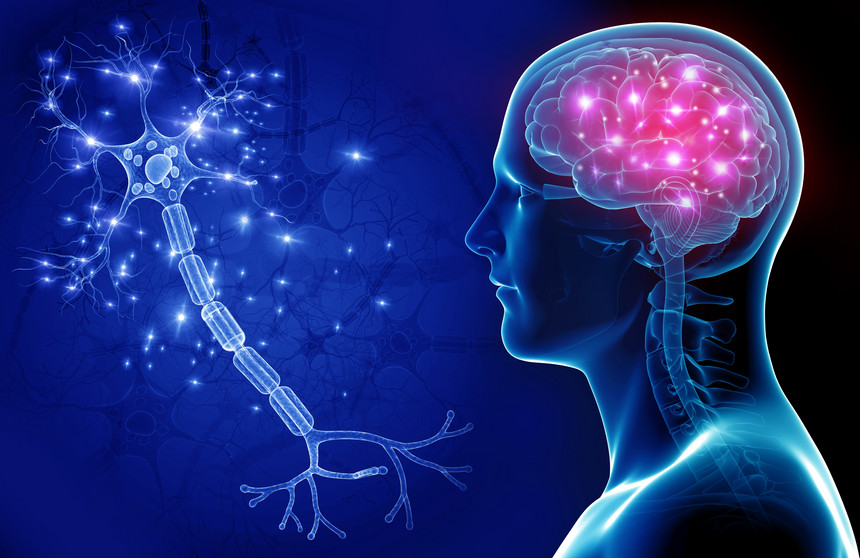
\includegraphics[width=0.9\textwidth]{modelo-monografia-rej-2018/img/mw-860.jpg}
    \caption{Cérebro e neurônio}
    \label{fig:Neuro}
    \end{figure}
    
    \begin{figure}
    \centering
    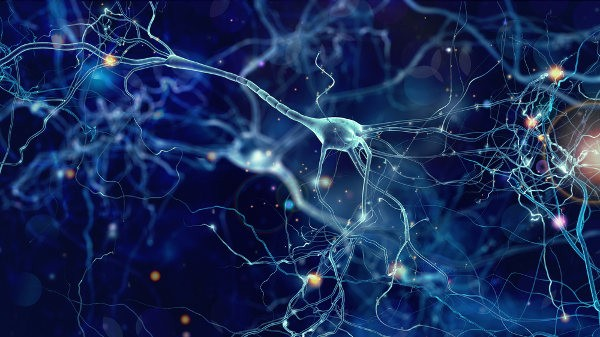
\includegraphics[width=0.9\textwidth]{modelo-monografia-rej-2018/img/neuronio.jpg}
    \caption{Neurônio}
    \label{fig:Neuronio}
    \end{figure}

\subsubsection{Neurônios Artificiais e a Rede Neural Artificial}

 \begin{citacao}
     Uma rede neural é um processador maciçamente paralelamente distribuído constituído de unidades de processamento simples, que têm a propensão natural para armazenar conhecimento experimental e torná-lo disponível para o uso. Ela se assemelha ao cérebro em dois aspectos: Conhecimento adquirido pela rede, através de um processo de aprendizagem, e forças de conexão entre neurônios, conhecidos como pesos sinápticos, usados para armazenar o conhecimento adquirido. \citeonline{haykin2001redes}
 \end{citacao}
 
\citeonline{haykin2001redes} descreveu ainda que a arquitetura de uma rede neural restringe o tipo de problema no qual a rede poderá ser utilizada, e é definida pelo número de camadas (camada única ou múltiplas camadas), pelo número de nós em cada camada, pelo tipo de conexão entre os nós (\textit{feedforward} ou \textit{feedback}) e por sua topologia.

Uma rede neural extrai seu poder computacional através de sua estrutura maciçamente paralelamente distribuída e de sua habilidade de aprender e portanto de generalizar --- refere-se ao fato de a rede neural produzir saídas adequadas para entradas que não estavam presentes durante o treinamento (aprendizagem). O uso de redes neurais fornecem algumas propriedades úteis e capacidades, são elas:

    \begin{enumerate}
        \item Não-linearidade:
        \item Mapeamento de Entrada-Saída:
        \item Adaptabilidade:
        \item Resposta à Evidências:
        \item Informação Contextual:
        \item Tolerância a Falhas:
        \item Implementação em VLSI -- \textit{Very-large-scale-integration}
        \item Uniformidade de Análise de Projeto:
        \item Analogia Neurobiológica
    \end{enumerate}
    
    Como dito anteriormente, o neurônio é uma unidade de processamento de informação que é fundamental para a operação de uma rede neural. A \autoref{fig:MoudeloNeuroNL} mostra o modelo de um neurônio, que forma a base para o projeto de redes neurais artificiais. Três elementos podem ser identificados na ilustração:
    \begin{itemize}
        \item Um conjunto de sinapses ou conexões, caracterizada por um ``peso''. O sinal de entrada é multiplicado pelo peso sináptico.
        \item Um somador para somar os sinais de entrada, ponderados pelas respectivas sinapses do neurônio; Um combinador linear.
        \item Uma função de ativação para restringir a amplitude da saída de um neurônio. É também referida como função restritiva já que limita o intervalo permissível de amplitude do sinal de saída a um valor finito.v"
        \item A figura inclui também um \textit{bias} aplicado externamente, que tem o efeito de aumentar ou diminuir a entrada líquida da função de ativação, dependendo se ele é positivo ou negativo, respectivamente. 
    \end{itemize}
    
    Um neurônio \textit{k} pode ser descrito matematicamente pelo par de equações \ref{eq:uk} e \ref{eq:yk}. Onde ${x_{1}, x_{2}, ..., x_{m}}$ são os sinais de entrada; ${w_{k1}, x_{k2}, ..., x_{km}}$; ${u_{k}}$ é a saída do combinador linear; ${b_{k}}$ é o bias; $\varphi$ é a função de ativação; e ${y_{k}}$ é o sinal de saída do neurônio.
    
    \begin{figure}
    \centering
    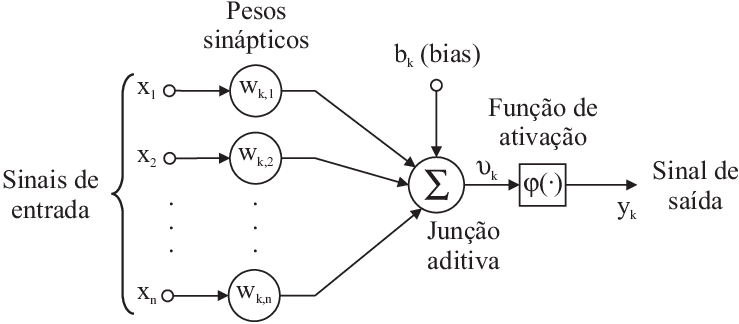
\includegraphics[width=0.9\textwidth]{modelo-monografia-rej-2018/img/Figura-1-Modelo-nao-linear-de-um-neuronio-Haykin-2001.png}
    \caption{Modelo não-linear de um neurônio}
    \label{fig:MoudeloNeuroNL}
    \end{figure}
    
    
    \begin{equation} \label{eq:uk}
        u_{k} = \sum_{j=1}^{m}{w_{kj}x_{j}}     
    \end{equation}
    
    \begin{equation} \label{eq:yk}
        y_{k} = \varphi (u_{k}+b_{k})
    \end{equation}
    
\subsubsection{Arquitetura de Rede}
A maneira pela qual os neurônios de uma rede neural estão estruturados está intimamente ligado com o algoritmo de aprendizagem usado para treinar a rede. Em geral, podemos identificar três classes de arquiteturas de rede diferentes:
    \begin{itemize}
        \item Redes Alimentadas Adiante com Camada Única: A forma mais simples de uma rede em camadas, temos a entrada de nós sobre uma camada de saída de neurônios, mas não vice-versa. Essa rede é chamada de Rede de Camada Única, referindo-se a camada saída de nós computacionais. A ilustração (a) na \autoref{fig:SLPMLP} apresenta uma rede acíclica de camada única.
        \item Redes Alimentadas Diretamente com Múltiplas Camadas: Se distingue pela presença de uma ou mais camadas ocultas. A função dos neurônios ocultos é intervir entre a entrada externa e a saída da rede de uma maneira útil. A ilustração (b) na \autoref{fig:SLPMLP} apresenta uma rede de camadas ocultas, com 10 nós de entrada, 4 camadas ocultas e 2 nós de saída, sendo assim uma rede 10-4-2.
        \item Rede Recorrentes: Se distinguem das duas anteriores por ter pelo menos um laço de realimentação. Uma rede recorrente pode consistir de uma única camada de neurônio com cada neurônio alimentando seu sinal de saída de volta para as entradas.
    \end{itemize}
    
    \begin{figure}
    \centering
    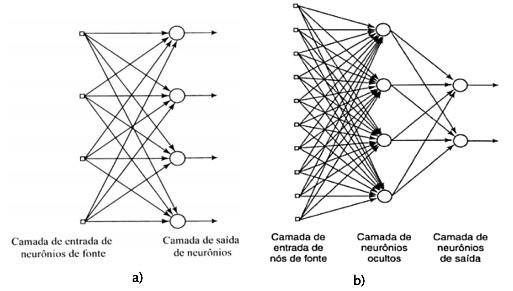
\includegraphics[width=0.9\textwidth]{modelo-monografia-rej-2018/img/Figura-1-a-Rede-de-camada-unica-b-Rede-de-multiplas-camadas.png}
    \caption{Redes Neurais de Camada Única e Múltiplas}
    \label{fig:SLPMLP}
    \end{figure}

\subsubsection{Aprendizagem}
A propriedade que é primordial para uma rede neural é a sua habilidade de aprender e de melhorar o seu desempenho através da aprendizagem. Segundo \citeonline{mendel19708}, a aprendizagem é um processo pelo qual parâmetros livres de uma rede neural são adaptados através de um processo de estimulação pelo ambiente. O tipo de aprendizagem é determinado pela maneira pela qual a modificação ocorre. Um conjunto preestabelecido de regras bem-definidas para a solução de um problema de aprendizagem é chamado de Algoritmo de aprendizagem. Basicamente, os algoritmos diferem entre si pela formulado o ajuste de um peso sináptico de um neurônio. 

Essa definição do processo de aprendizagem implica  a seguinte sequência de eventos:
    \begin{enumerate}
        \item A rede neural é estimulada por um ambiente.
        \item A rede neural sofre modificações nos seus parâmetros livres como resultado desta estimulação.
        \item A rede neural responde de uma maneira nova ao ambiente, devido às modificações ocorridas na sua estrutura interna.
    \end{enumerate}
  
%https://www.maxwell.vrac.puc-rio.br/7587/7587_5.PDF
%http://www.ic.uff.br/~jsilva/monografia_RNA.pdf

\subsubsubsection{Aprendizagem por Correção de Erro}
Neste modelo a correção dos pesos sinápticos é efetuada através da comparação da saída desejada com a saída atual, ambas medidas no mesmo instante de tempo. O erro é então definido com sendo a diferença do valor da saída desejado e a saída atual.

A fim de se estimar o erro da rede define-se uma função custo baseada na função erro. Esta função indica o erro instantâneo da rede e procura-se em adaptar os pesos
sinápticos a fim de minimizar essa função. 

\begin{equation} \label{eq:erro}
    e_{k}(n) = d_{k}(n) - y_{k}(n)    
\end{equation}

A \autoref{eq:erro} descreve a função de erro, onde o sinal de erro $e_{k}(n)$ aciona um mecanismo de controle, com propósito de aplicar uma sequência de ajustes corretivos aos pesos sinápticos do neurônio k. Os ajustes corretivos são projetados para aproximar passo a passo o sinal de saída $y_{k}(n)$ da resposta desejada $d_{k}(n)$. O objetivo é alcançado minimizando-se uma função de custo ou índice de desempenho, E(n), definido em termos do sinal de erro $e_{k}(n)$ como descrito na \autoref{eq:custo}. $E(n)$ é o valor instantâneo da energia do erro. Os ajustes dos pesos sinápticos continuam até o sistema atingir um estado estável.

\begin{equation} \label{eq:custo}
    E(n) = \frac{1}{2}e_{k}^{2}(n)
\end{equation}

A minimização da função de custo $E(n)$ resulta na \textbf{Regra Delta} ou \textbf{Regra de Widrow-Hoff}, denominada em homenagem aos criadores \cite{widrow1960adaptive}. Supondo que $w_{kj}(n)$ represente o valor do peso sináptico $w_{kj}$ do neurônio k estimulado por um elemento $x_{j}(n)$ do vetor de sinal $\textbf{x}(n)$ no passo de tempo n. De acordo com a regra delta, o ajuste $\Delta w_{kj}(n)$ aplicado aos peso sináptico no tempo n é definido por:

\begin{equation} \label{eq:delta}
    \Delta w_{kj}(n) = \eta e_{k}(n)x_{j}(n)
\end{equation}

Na \autoref{eq:delta}, $\eta$ é uma contante positiva que determina a taxa de aprendizado quando avançamos em um passo no processo de aprendizagem. A regra delta pode ser formulada como: 
    
    \begin{citacao}
        O ajuste feito em um peso sináptico de um neurônio é proporcional ao produto do sinal de erro pela sinal de entrada da sinapse em questão. \cite{haykin2001redes}
    \end{citacao}

Após o calculo do ajuste sináptico $\Delta w_{kj}(n)$, o valor atualizado do peso sináptico $w_{kj}(n)$ é determinado pela  \autoref{eq:atualPeso}

\begin{equation} \label{eq:atualPeso}
    w_{kj}(n+1) = w_{kj}(n) + \Delta w_{kj}(n)
\end{equation}

\subsubsubsection{Aprendizagem baseada em Memória}
Na aprendizagem baseada em memória, todas as (ou a maioria das) experiências passadas são armazenadas em uma grande memória de exemplos de entrada-saída classificados corretamente: $\left \{ \left ( \textbf{x}_{i}, d_{i} \right ) \right \}_{i=1}^{N}$, onde $\textbf{x}_{i}$ representa um vetor de entrada e $d_{i}$ representa a resposta desejada correspondente. Todos os algoritmos de aprendizagem baseada em memória envolvem dois elementos essenciais:
    
    \begin{itemize}
        \item O critério utilizado para definir a vizinhança local do vetor de teste $\textbf{x}_{teste}$
        \item A regra de aprendizagem aplicada aos exemplos de treinamento na vizinhança local de teste $\textbf{x}_{teste}$
    \end{itemize}

\subsubsubsection{Aprendizagem Hebbiana}
O postulado de aprendizagem de Hebb é a mais antiga e mais famosas das regras de aprendizagem, sendo denominada em homenagem ao neuropsicólogo \citeonline{hebb1949organization}. 

    \begin{citacao}
        Quando um axônio da célula A está perto o suficiente para estimular uma célula B e participa do seu disparo repetida ou persistentemente, então algum processo de crescimento ou modificação metabólica acontece em uma das células ou em ambas,de tal forma que a eficiência de A como uma das células que dispara B é aumentada.
    \end{citacao}
    
    A proposta foi feita como uma base da aprendizagem associativa (a nível celular), que resultaria em uma modificação permanente do padrão de atividade de um ``agrupamento de células neervosas'' espacialmente distribuído. A afirmação foi feita em um contexto neurobiológico. Pode-se expandir e reescrevê-la como uma regra em duas partes (\citeonline{stent1973physiological}; \citeonline{changeux1976selective}):
    \begin{enumerate}
        \item Se dois neurônios em ambos os lados de uma sinapse (conexão) são ativados simultaneamente, então a força daquela sinapse é seletivamente aumentada.
        \item Se dois neurônios em ambos os lados de uma sinapse são ativados assincronamente, então aquela sinapse é seletivamente enfraquecida ou eliminada.
    \end{enumerate}

Uma sinapse assim é denominada sinapse hebbiana. (A regra de Hebb original não contém a parte 2). A sinapse hebbiana pode ser definida como uma sinapse que usa um mecanismo dependente do tempo, altamente local e fortemente interativo para aumentar a eficiência sináptica como uma função da correlação entre as atividades pré-sinápticas e pós-sináptica.
A aprendizagem hebbiana é definida em termos matemáticos, considerando um peso sináptico $w_{kj}$ do neurônio k com sinais pré-sinápticas e pós-sináptica representados por $x_{j}$ e $y_{k}$, respectivamente. O ajuste aplicado ao peso sináptico $w_{kj}$ no passo de tempo n é expresso na forma geral:

\begin{equation} \label{eq:hebb1}
    \Delta w_{kj}(n) = F(y_{k}(n), x_{j}(n))
\end{equation}

onde F(,) é uma função tanto do sinal pré-sinápticas como do pós-sináptico. A forma mais simples de aprendizagem hebbiana é descrita por:

\begin{equation} \label{eq:hebb2}
    \Delta w_{kj}(n) = \eta y_{k}(n), x_{j}(n)
\end{equation}

A aplicação repetida do sinal de entrada $x_{j}$ resulta em um aumento de $y_{k}$ e, portanto, em um crescimento exponencial que ao final leva a conexão sináptica à saturação. Naquele ponto nenhuma informação será armazenada na sinapse e a seletividade é perdida. Uma forma de superar a limitação da hipótese de Hebb é através da utilização da hipótese de covariância introduzida por \citeonline{sejnowski1977storing}, que os sinais pré-sinápticos e pós-sinápticos da \autoref{eq:hebb2} são substituídos pelo desvio dos sinais em relação aos seus respectivos valores médios em um certo intervalo de temo. O ajuste aplicado ao peso sináptico é definido por:

\begin{equation} \label{eq:hebb2}
    \Delta w_{kj}(n) = \eta(x_{j} - \bar{x})(y_{k} - \bar{y})
\end{equation}

onde $\eta$ é o parâmetro taxa de aprendizado. Os valores $\bar{x}$ e $\bar{y}$ são valores médios no tempo dos sinais $x_{k}$ e $y_{k}$, respectivamente.

\subsubsubsection{Aprendizagem Competitiva}
Na aprendizagem competitiva, os neurônios de saída de uma rede neural competem entre si para se tornar ativos (disparar). Diferente de uma rede neural baseada em aprendizagem hebbiana, onde vários neurônios de saída podem estar ativos simultaneamente, na competitiva somente um único neurônio de saída está ativo em um determinado instante. Essa característica torna a aprendizagem competitiva muito adequada para descobrir características estatisticamente salientes que podem ser utilizadas para classificar um conjunto de padrões de entrada. Existem três elementos básicos em uma regra de aprendizagem competitiva \cite{rumelhart1985feature}:
    \begin{itemize}
        \item Um conjunto de neurônios são todos iguais entre si, exceto por alguns pesos sinápticos distribuídos aleatoriamente, e que por isso respondem diferentemente a um dado conjunto de padrões de dados.
        \item Um limite imposto sobre a força de cada neurônio.
        \item Um mecanismo que permite que o neurônio compita pelo direito de responder a um dado subconjunto de entradas, de forma que somente um neurônio de saída, ou somente um neurônio por grupo esteja ativo em um determinado instante.
    \end{itemize}
    
    Podemos escrever o sinal de saída $y_{k}$ de um neurônio k como 1, para o vencedor, e 0, para os neurônios que perderam a competição, como descrito a seguir:
    
    \begin{equation}
        \left\{\begin{array}{ll}1,\ se\ v_{k} > v_{j}\ para\ todos\ j,\ j \neq k\\0,\ caso\ contrário \end{array}\right.
    \end{equation}
    
    onde $v_{k}$ representa a ação combinada de todas as entradas diretas e realimentadas do neurônio k.
    
    Os pesos sináptico da conexão do nó de entrada j ao neurônio k pode ter alocado uma quantidade fixa em cada neurônio, sendo distribuída para os nós de entrada. 
    
    Um neurônio, então, aprende ao deslocar pesos sinápticos de seus nós de entrada inativos para os seu nós ativos. Seu um neurônio não responde a um padrão de entrada particular, então cada nó de entrada deste neurônio libera uma certa proporção de seu peso sináptico e esse peso será então distribuído uniformemente entre os nós de entrada ativos. De acordo com a regra de aprendizagem competitiva padrão, a variação $Delta w_{kj}$ aplicada ao peso sináptico $w_{kj}$ é definida por:
    
    \begin{equation} \label{eq:boltz}
        \Delta w_{kj} = \left\{\begin{array}{ll}\eta(x_{j} - w_{kj}),\ se\ o\ neurônio\ k\ vencer\ a\ competição\\0,\ se\ o\ neurônio\ k\ perder\ a\ competição \end{array}\right.
    \end{equation}
    
\subsubsubsection{Aprendizagem de Boltzmann}
A regra de aprendizagem de Boltzmann, em homenagem a Ludwig Boltzmann, é um algoritmo de aprendizagem estocástico derivado de ideias
enraizadas na mecânica estatística. Uma rede neural projetada com base na regra de aprendizagem de Boltzmann é denominada uma máquina de Boltzmann \cite{ackley1985learning}. 

Em uma máquina de Boltzmann, os neurônios constituem uma estrutura recorrente e operam de uma maneira binária, uma vez que eles estão em um estado ``ligado'' ou ``desligado'', representados por 1 e -1, respectivamente. A máquina é caracterizada por uma função de energia, E, cujo valor é determinado pelos estados particulares ocupados pelos neurônios individuais da máquina, sendo escrito da seguinte forma:
    
    \begin{equation}
        E = -\frac{1}{2}{\sum_{j}\sum_{k}}_{j \neq k}w_{kj}x_{k}x_{j}
    \end{equation}
    
    onde $x_{j}$ é o estado do neurônio j e $w_{kj}$ é o peso sináptico conectando o neurônio j ao neurônio k.
    
\subsubsubsection{Aprendizagem Supervisionada}
A aprendizagem supervisionada, também denominada aprendizagem com um professor, é um paradigma de aprendizagem, onde uma ``entidade'' - um ``professor'' - tem um conhecimento sobre o ambiente, com este conhecimento sendo representado por um conjunto de exemplos de entrada-saída. Entretanto, o ambiente é desconhecido pela rede neural de interesse. 

Dado um vetor de treinamento (i.e., exemplo) retirado do ambiente, em virtude do conhecimento prévio, o professor é capaz de fornecer à rede neural uma resposta esperada, a ação ótima. Os parâmetros da rede são ajustados sob a influência combinada do vetor de treinamento e do sinal de erro. O sinal de erro é definido como a diferença entre a diferença entre a resposta desejada e a resposta real da rede. O ajuste é realizado iterativamente, com objetivo de fazer a rede neural emular o professor.

Como uma medida de desempenho para o sistema, pode-se pensar em termos do erro médio quadrado ou da soma de erros quadrados sobre a amostra de treinamento, definida como uma função dos parâmetro livres do sistema. Esta função pode ser visualizada como uma superfície multidimensional de desempenho de erro, com os parâmetros livres como coordenadas.

\subsubsubsection{Aprendizagem sem um professor}
Na aprendizagem supervisionada, visto anteriormente, o processo de aprendizagem acontece sob a tutela de um professor. Já no paradigma conhecido como aprendizagem sem um professor, onde não há um professor para supervisionar o processo de aprendizagem. Ou seja, não há exemplos rotulados da função a ser aprendida pela rede.

\begin{enumerate}
\item \textbf{Aprendizagem por reforço/Programação Neurodinâmica}

Na aprendizagem por reforço, o aprendizado de um mapeamento de entrada-saída é realizado através da interação contínua com o ambiente, visando a minimizar um índice escalar de desempenho. O sistema é projetado para aprender por reforço atrasado, o que significa que o sistema observa uma sequência temporal de estímulos recebidos do ambiente, que eventualmente resultam na geração do sinal de reforço heurístico. O objetivo da aprendizagem é minimizar uma função de custo para avançar, definida como a expectativa do custo cumulativo de ações tomadas ao longo de uma sequência de passos.

\item \textbf{Aprendizagem Não-Supervisionada}

Na aprendizagem não-supervisionada ou auto-organizada, não há um professor externo ou um crítico para supervisionar o processo de aprendizado. Em vez disso, são dadas condições para realizar uma medida independente da tarefa da qualidade da representação que a rede deve aprender, e os parâmetros livre da rede são otimizados em relação a esta medida. Uma vez que a rede tenha se ajustado às regularidades estatísticas dos dados de entrada, ela desenvolve a habilidade de formar representações internas para codificar as características da entrada e, desse modo, de criar automaticamente novas classes \cite{becker1991unsupervised}.

Para realizar a aprendizagem não-supervisionada, pode-se utilizar a regra de aprendizagem competitiva. Por exemplo, pode-se usar uma rede neural de duas camadas -- uma camada de entrada e uma camada competitiva. A camada de entrada recebe os dados disponíveis. A camada competitiva consiste de neurônios que competem entre si.
\end{enumerate}

\subsubsection{Perceptron de Camada Única}
O Perceptron é a forma mais simples de uma rede neural usada para a classificação de padrões ditos linearmente separáveis (i.e., padrões que se encontram em lados opostos de um um hiperplano). Basicamente, ele consiste de um único neurônio com pesos sinápticos ajustáveis e bias. O algoritmo usado para ajustar os parâmetros livres desta rede neural apareceu primeiro em um procedimento de aprendizagem por \citeonline{rosenblatt1958perceptron} para o seu modelo cerebral do perceptron. O perceptron construído em torno de um único neurônio é limitado a realizar classificação de padrões com apenas duas classes (hipóteses). Expandindo a camada de (computação) saída do perceptron para incluir mais de um neurônio, podemos correspondentemente realizar classificação com mais de duas classes. 

O neurônio único também forma a base de um filtro adaptativo, um bloco funcional que é básico para o tema do processamento de sinais. O desenvolvimento da filtragem adaptativa deve muito ao clássico artigo de \citeonline{widrow1960adaptive}, por criar o Algoritmo do mínimo quadrado médio (LMS, \textit{Least-mean-square}), também conhecido como Regra delta (\autoref{eq:delta}).

\subsubsection{Perceptron de Múltiplas Camadas}
Tipicamente, a rede consiste de um conjunto de unidades sensoriais (nós de fonte) que constituem a camada de entrada, uma ou mais camadas ocultas de nós computacionais e uma camada de saída de nós computacionais. O sinal de entrada se propaga para frente através da rede, camada por camada. Estas redes são chamadas de perceptron múltiplas camadas (MLP, \textit{Multilayer perceptron}). 

Os perceptrons de múltiplas camadas têm sido aplicados com sucesso para resolver diversos problemas difíceis, através do seu treinamento de forma supervisionada com um algoritmo, conhecido como algoritmo de retro propagação de erro (\textit{error back-propagation}), que é baseado na regra de aprendizagem por correção de erro. 

Basicamente, a aprendizagem por retro-propagação de erro consistem de dois passos através das diferentes camadas da rede: um passo para frente, a propagação, e um passo pra trás, a retro-propagação. Na propagação, um padrão de atividade (vetor de entrada é aplicado aos nós sensoriais da rede e seu efeito se propaga através da rede. Finalmente, um conjunto de saídas é produzido como a resposta real da rede, sendo os pesos sinápticos da rede fixos. Durante o passo para trás, os pesos sinápticos são todos ajustados de acordo com uma regra de correção de erro. O perceptron de múltiplas camadas usa uma variação da regra delta, a regra delta generalizada. A regra delta generalizada funciona quando são utilizadas na rede unidades com uma função de ativação semi-linear, que é uma função diferenciável e não decrescente. Uma função de ativação amplamente utilizada, nestes casos, é a função sigmoide. A regra delta generalizada pode ser definida como: {\color{red} A CONFIRMAR}

\begin{equation}
    E_{j} = \frac{1}{2} \sum_{i=1}^{n} (d_{j} - s_{j})^{2}
\end{equation}

\begin{equation}
    \Delta w_{kj}^{s}(n) = \eta \delta_{k}^{s}(n) i_{j}(n) + \alpha \Delta w_{kj}^{s} (n-1)
\end{equation}

\begin{equation}
    E(w) = \frac{1}{2}\sum_{l=1}^{L}(f(w^{t}x_{l}^{d})-y_{l}^{d})^{2}
\end{equation}

Gradiente:

\begin{equation}
    \nabla E[\vec{w}] = \left [ \frac{\partial E}{\partial w_{0}}, \frac{\partial E}{\partial w_{1}}, ..., \frac{\partial E}{\partial w_{n}} \right ]
\end{equation}

Regra de treinamento:

\begin{equation}
    \Delta \vec{w} = -\eta \nabla E [\vec{w}]
\end{equation}

i.e.,

\begin{equation}
    \Delta \vec{w_{i}} = -\eta \left [ \frac{\partial E}{\partial w_{i}} \right ]
\end{equation}

\begin{equation}
    \left [ \frac{\partial E}{\partial w_{i}} \right ] = \sum_d (t_{d} - O_{d})(x_{i,d})
\end{equation}

\subsubsection{Processamento de entrada e Algoritmo de Treinamento}
{\color{red}TEXTO}

\subsubsection{Avaliação de RNA}
A RNA pode ser avaliada em relação à sua Precisão, Acurácia e Recall.
{\color{red}MELHORAR TEXTO}

\subsubsubsection{Acurácia}
{\color{red}TEXTO}
\textbf{Acurácia} se define como a proximidade da medida em relação ao verdadeiro valor, um valor definido, que se deseja obter. Quanto mais próximo do valor real, melhor é a acurácia. A \autoref{fig:PrecAcur} esclarece isso de maneira bem didática.

\subsubsubsection{Precisão}
{\color{red}TEXTO}
\textbf{Precisão} se define como a proximidade entre os valores obtidos pela repetição do processo de mensuração. Quanto menor é a diferença destes valores, melhor é a precisão. 
\subsubsubsection{\textit{Recall}}
{\color{red}TEXTO}

\begin{figure}
    \centering
    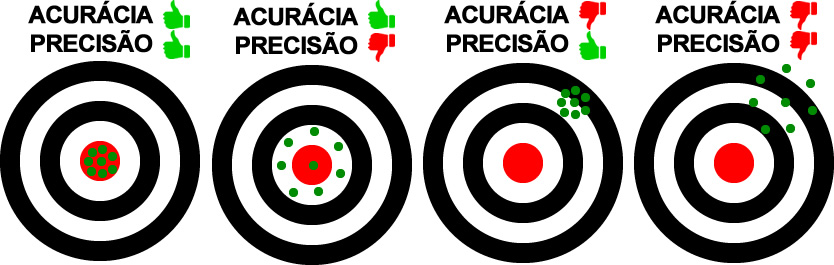
\includegraphics[width=0.9\textwidth]{modelo-monografia-rej-2018/img/PrecisaoAcuracia.jpg}
    
    \caption{Diferença entre Acurácia e Precisão}
    \label{fig:PrecAcur}
\end{figure}

\section{Aprendizagem Baseada em jogos - \textit{Games-based Learning}}
\label{sec:GBL}

Aprendizagem Baseada em jogos, ou GBL (pela sigla em inglês de \textit{Games-based Learning}), foi definida por alguns autores. Segundo \citeonline{tang2009introduction}, GBL faz referência a uma abordagem de aprendizagem inovadora derivada do uso de jogos de computador que tem valor educacional ou diferentes tipos de aplicação de software que usam jogos computacionais para ensino e educação. GBL's têm como finalidade o apoio à aprendizagem, a avaliação e análise de alunos e melhoria do ensino. Segundo \citeonline{monsalve2014aprendizagem}, aprendizagem baseada em jogos surge como uma alternativa de ensino que se adapta às características da pedagogia moderna na qual o estudante é um ator ativo.

Para \citeonline{monsalve2011teaching}, com a aprendizagem baseada em jogos, se pretende equilibrar entretenimento e difusão do conhecimento, motivando os estudantes a aprender enquanto jogam. \citeonline{Souza:2017:GLB:3103028.3103054} definiram \textit{GBL} como o ato de aplicar jogos com o propósito de aprender habilidades e conceitos específicos, geralmente nomeado como “jogos sérios” (jogos com fins), entretenimento educativo\footnote{Do termo, em inglês, “\textit{Edutainment}”, que seria a união de educação (\textit{Education}) e entretenimento (\textit{entertainment})} ou jogos educativos. Já \citeonline{von2009game} definiram GBL como uma abordagem lida com aplicativos de jogos que definiram resultados de aprendizagem.

Algumas plataformas de GBL foram utilizadas por autores no processo de ensino-aprendizagem. Um destes foi o de \citeonline{lot2016game}, onde abordaram o uso de GBL como avaliação formativa, com a plataforma \textbf{Zoondle}. Outras plataformas de GBL usadas foram a \textbf{EducaCross}, no trabalho de \citeonline{reis2016experiencia}, a \textbf{Timemesh}, no trabalho de \citeonline{baptista2013timemesh} e, provavelmente o mais popular, \textbf{Kahoot!}, que será usado neste projeto de pesquisa {\color{red}[Por quê escolher o Kahoot? Referenciar.]}.

\subsection{Kahoot!} \label{sec:Kahoot!}
Kahoot! é uma plataforma de aprendizado baseada em jogos usada como tecnologia educacional em escolas, universidades e outras instituições de ensino. Kahoot! foi fundada por Johan Brand, Jamie Brooker e MortenVersvik em um projeto conjunto com a Universidade Norueguesa de tecnologia e ciência \cite{kahoot2018}. Seus jogos de aprendizado, ``Kahoots'', são \textit{quizzes}, perguntas de múltipla escolha, que permitem a criação de usuários e podem ser acessados por meio de um navegador da Web, telefone ou pelo aplicativo.

Kahoot! foi projetado para a aprendizagem social, com os alunos reunidos em torno de uma tela comum, como um quadro interativo, projetor ou um monitor de computador. O site também pode ser usado por meio de ferramentas de compartilhamento de tela, como Skype ou Google hangouts. Kahoot! pode ser usado para revisar o conhecimento dos alunos, para avaliação formativa \cite{kahootFormative}, ou como uma pausa com as atividades tradicionais em sala de aula. 

A jogabilidade é simples; todos os jogadores se conectam usando um PIN de jogo gerado na tela comum e usam um dispositivo para responder a perguntas criadas pelo professor. As questões podem ter pontuações atribuídas em relação ao acerto e ao tempo para resposta. Os pontos aparecem no placar depois de cada pergunta.

Alguns trabalhos relataram os resultados encontrados ao utilizar o Kahoot! no processo de ensino. Um destes foi realizado por \citeonline{diniz2018kahoot}, que usou a ferramenta com alguns alunos de Ciência da Computação, obtendo resultados satisfatórios quanto a aceitação da ferramenta no contexto educacional.

\begin{comment}
%Artigos complementares
{\color{red}LER}
    
    \cite{chaiyo2017effect}\\
    \cite{tobias2014game}\\
    \cite{wang2015wear}\\
    \cite{connolly2012systematic}\\
    \cite{backlund2013educational}
\end{comment}
 
 No trabalho de \citeonline{petri2016quiz}, o Kahoot! foi utilizado como um \textit{quiz} com perguntas sobre Gerenciamento de Projetos, disponibilizado para alunos dos cursos de Sistemas de
Informação e Ciência da Computação como forma de revisão de conteúdo. Os autores identificaram \textit{feedbacks} positivos nos resultados encontrados. Afirmaram também que o jogo educacional cumpriu com o seu objetivo de aprendizagem por proporcionar a revisão de conhecimentos de forma divertida e motivadora.

Para os autores \citeonline{abidin2017students}, a utilização do Kahoot! foi uma estratégia de motivação para os alunos de uma faculdade de Engenharia Elétrica ao cursarem uma disciplina de programação de computadores. O conteúdo apresentado no \textit{game} era relacionado a disciplina em questão e o objetivo era possibilitar aos alunos uma experiência atrativa para a aprendizagem, pois muitos deles perdiam o entusiamo ao estudarem programação de computadores. O resultado mostrou que a grande maioria dos alunos conseguiu melhorar sua  compreensão sobre a disciplina e também se mostraram mais engajados e motivados ao final do experimento.

Outro trabalho similar foi o realizado por \citeonline{correia2017game}, que apresenta as opiniões de alunos de um programa de formação de professores (licenciatura e mestrado) sobre as vantagens e desvantagens da utilização do Kahoot! em sala de aula. Como vantagens percebidas estão a correção automática das questões e o \textit{feedback} em tempo real para os alunos e professores. Como desvantagens, foram identificados os seguintes fatores: numero limitado de caracteres tanto para o enunciado das questões quanto para as opções de respostas, além do tempo limitado de resposta.

 Considerando que alguns fatores sociais e geográficos podem afetar a aplicação e a eficiência do uso desta ferramenta, faz-se necessário avaliá-la no contexto dos estudantes brasileiros. Segundo \citeonline{pintor2014kahoot}, Kahoot! mantém as mesmas utilidades que outros métodos de resposta rápida; especialmente os \textit{clickers}, mas sem todos os problemas técnicos e logísticos destes.

\begin{comment}
\section{Introdução}
\indent\indent Este capítulo apresenta as principais características para construção de uma monografia. O referencial teórico do tema é apresentado nesta seção, ou seja, todo o conceito do trabalho deve ser descrito indicando por meio de referências, as bibliografias dos trabalhos que foram publicados sobre o tema, e que permitem o autor conceituar o assunto.
\section{Formatação da monografia}
\indent Os textos devem ser apresentados em papel branco, formato A4. Deverá ser digitado em tinta cor preta, com exceção de ilustrações. As folhas deverão apresentar margem esquerda e superior de 3 cm; direita e inferior de 2 cm. De forma geral este modelo (template) apresenta todas formatações necessárias. 
A tabela \ref{tab1} é um exemplo. 


\begin{table}[htp]
\caption{Modelo de Tabela com referência \cite{hancock1995virtual}}  
 \begin{center}
  \begin{tabular}{c|c|c|c}
   \hline
   Características & C1 & C2 & C3 \\
   \hline
   1000 & 2000 & 3000 & 1000 \\
   4000 & 2000 & 3000 & 1000 \\
   5000 & 3000 & 1000 & 1000 \\
   \hline
  \end{tabular}
  \label{tab1}
 \end{center}
\end{table}

 
\indent Tabela \ref{tab1} mostra .....

\begin{figure}[htp]
\centering

\includegraphics[scale=0.9]{img/ModeloImagem.jpg}
\caption{Modelo de Imagem \cite{pimentel1995}}
\label{modeloimg}
\end{figure}
 
	A Figura \ref{modeloimg} mostra um exemplo de como inserir uma imagem/figura e como fazer referência bibliográfica a mesma. 


Segundo \citeonline{marcoswagner_tese}, um exemplo de itens pode ser visto abaixo:

	\begin{itemize}
		\item Quanto as características da lesão:
		
	\begin{itemize}
		\item Tempo em que ocorreu a lesão:
		\item Extensão da lesão.
		\item Local da lesão.
	\end{itemize}
		\item Biografia do paciente:
		\item Idade.
		\item Diagnóstico. 
		\item Início e duração da terapia.
		\item Frequência e intensidade da terapia.
		\item Estado emocional.
		\begin{itemize}
			\item Motivação.
			\item Depressão.
		\end{itemize}
		\item Ambiente terapêutico.
		\item Comunicação.
		\item Condições físicas.
		\item Cognição; e
		\item Programa terapêutico.
	\end{itemize}




\section{Considerações Finais}
Tanto a seção Introdução como a seção Considerações Finais são opcionais na construção de um texto monográfico. Porém deve-se optar por um padrão. Coloca-se em todos os capítulos ou em nenhum...


\end{comment}


\chapter{Trabalhos relacionados}\label{cap:relacionados}
No decorrer dessa pesquisa foram encontrados alguns trabalhos que propõem métodos para a predição de desempenho acadêmico. Nesta seção, serão apresentados do levantamento bibliográfico feito para encontrar esses trabalhos, os trabalhos correlatos que estão fortemente ligados com este projeto de pesquisa, seguido de breve resumo do que cada autor propôs e obteve como resultado, e uma tabela apresentado as  características de cada um dos trabalhos.

\section{Levantamento Bibliográfico} \label{sec:Lev}
Foi realizado um levantamento bibliográfico para recuperar trabalhos correlatos realizados por outros autores, para apoiar as afirmações e explanações a serem desenvolvidas.

%Objetivos
\subsection{Objetivo}
\label{sec:Obj}
O objetivo deste levantamento bibliográfico é fazer uma revisão, seleção e organização dos artigos que possam identificar os alunos em situação de risco, analisando os métodos propostos.

%Questões de pesquisa
\subsection{Questões de Pesquisa}
\label{sec:QP}
Para nortear esta levantamento, foram definidas questões que elenquem pontos relevantes a serem estudados.
\begin{itemize}
    \item \textbf{Questão 1}: Quais métodos foram propostos para identificar alunos com risco de reprovação em disciplinas?
    \item \textbf{Questão 2}: Quais os graus de precisão e acurácia alcançados ao utilizar-se destes métodos?
    \item \textbf{Questão 3}: Redes Neurais Artificias foram utilizadas? Se sim, são assertivas na predição de alunos em situação de risco?
    \item \textbf{Questão 4}: Quais são as vantagens de se utilizar Redes Neurais Artificiais para tal?
\end{itemize}

\subsection{Método de pesquisa} \label{sec:MP}
Nesta seção serão descritos alguns elementos utilizados para o levantamento bibliográfico, de acordo com \citeonline{kitchenham2004procedures}. São estes: o escopo da pesquisa, o idioma considerado, os termos utilizados, a \textit{string} de busca e os critérios de seleção de artigos.


\subsubsection{Máquinas de busca utilizadas}
Para este levantamento bibliográfico, foram escolhidos três das principais máquinas de buscas disponíveis atualmente. Aplicou-se as \textit{Strings} de buscas - no período de 2013 a 2018 - que serão apresentadas mais a frente, a fim de identificar potenciais trabalhos correlatos ao tema deste. As máquinas de busca utilizadas para a pesquisa foram:

\begin{itemize}
    \item ACM Digital Library
    \item Google Scholar
    \item IEEE Xplore
\end{itemize}

\subsubsection{Idiomas dos Artigos}
Por se tratarem da língua oficial brasileira e uma das línguas mais faladas, respectivamente, Português e Inglês foram os idiomas escolhido para a pesquisa dos artigos.

\subsection{Palavras-chave e \textit{strings} de busca}

As palavras-chave que compõem a busca são (em português e inglês, respectivamente): 
Educação de Computação, Ensino de Computação, Introdução a Computação, Avaliação, Estimativa, Previsão, Inteligência Artificial, Mineração de Dados, Aprendizado em Profundidade, Redes Neurais Artificiais, RNA, \textit{Computer Education}, \textit{CS1}, \textit{Assessment}, \textit{Prediction}, \textit{Artificial Intelligence}, \textit{Data Mining}, \textit{Clicker}, \textit{Deep Learning}, \textit{Artificial Neural Network}, \textit{ANN}.

A \autoref{string-busca} mostra as \textit{strings} de busca foram geradas a partir da combinação das palavras chave, dividida pelos idiomas estabelecidos.

\begin{comment}
\begin{center}
\begin{longtable}{|| p{3cm} || p{10cm} ||}
\caption{String de Busca}
\label{string-busca}
\hline
\textit{\textbf{Português}} & (``Educação de computação'' OR ``ensino de computação'' AND ``Introdução a Computação'' OR ``Avaliação'') AND (``estimativa'' OR ``previsão'' AND ``Inteligência Artificial'' OR ``mineração de dados'' OR ``Aprendizado em Profundidade'' OR ``Redes Neurais Artificiais'' OR ``RNA'')\\
\hline \hline
\textit{\textbf{Inglês}} & \textit{(``Computer Education'' AND ``cs1'' OR ``assessment'') AND (``prediction'' OR ``data mining'' OR ``artificial intelligence'' OR ``deep learning'' OR ``Artificial neural network'' OR ``ANN''))}\\
 \hline \hline
\end{longtable}
\end{center}
\end{comment}

{\color{red} CORRIGIR TABELA}

\begin{table}[]
\caption{Strings de Busca}
\label{Strings}
\resizebox{\textwidth}{!}{%
\begin{tabular}{l|l}
\textit{\textbf{Português}} & \begin{tabular}[c]{@{}l@{}}(``Educação de computação'' OR ``ensino de computação'' AND \\ ``Introdução a Computação'' OR ``Avaliação'') AND \\ (``estimativa'' OR ``previsão'' AND ``Inteligência Artificial'' \\ OR ``mineração de dados'' OR ``Aprendizado em Profundidade'' \\ OR ``Redes Neurais Artificiais'' OR ``RNA'')\end{tabular} \\ \hline
\textit{\textbf{Inglês}} & \textit{\begin{tabular}[c]{@{}l@{}}(``Computer Education'' AND ``cs1'' OR ``assessment'') AND \\ (``prediction'' OR ``data mining'' OR ``artificial intelligence'' \\ OR ``deep learning'' OR ``Artificial neural network'' OR ``ANN''))\end{tabular}}
\end{tabular}%
}
\end{table}



\subsubsection{Critérios de Seleção de Artigos e Procedimentos}
\citeonline{kitchenham2004procedures} diz que devem ser seguidos critérios de inclusão e exclusão para os artigos que são retornados pela \textit{string} de busca. Sendo assim, foram definidos os seguintes critérios:

\subsubsection{Critérios para Inclusão de Artigos}

\begin{enumerate}
    \item Pesquisas as quais tratam sobre utilização de métodos para identificação de alunos em situação de risco de reprovação;
    \item Pesquisas as quais tratam sobre inteligência artificial no contexto educação de computação e no processo de ensino-aprendizagem;
    \item Pesquisas as quais tratam sobre previsão do desempenho acadêmico com uso de aprendizado de máquina.
\end{enumerate}

\subsubsection{Critérios para Exclusão de Artigos}
\begin{enumerate}
    \item Não apresentar necessidade de identificar os alunos em situação de riscos;
    \item Não apresentar a forma utilizada para coletar dados;
    \item Não apresentou os métodos utilizados para analisar os dados obtidos;
    \item Não foi possível ter acesso a pesquisa completa;
    \item A pesquisa não está disponível na \textit{web};
    \item A pesquisa é publicada apenas como resumo;
    \item Trabalhos que são réplicas ou continuações/evoluções de projetos de pesquisas iniciais, incluindo o trabalho mais completo (Geralmente, o mais recente);
    \item Ter sido publicado em período anterior a 2013.
\end{enumerate}

\subsection{Processo de triagem}
Foi realizada uma primeira triagem, que consistiu na leitura do título, do resumo (\textit{abstract}) e das palavras-chave (\textit{keywords}) dos trabalhos previamente recuperados, aplicando os critérios de inclusão e exclusão e as \textit{Strings} de busca.
A etapa seguinte teve como objetivo realizar a leitura completa e minuciosa dos artigos selecionados na primeira fase. Desta forma, a segunda fase do processo de triagem possibilita fazer uma análise mais apurada dos estudos, identificando e extraindo dados de acordo com os critérios de inclusão e exclusão descritos anteriormente.

\section{Trabalhos Relacionados selecionados}
Após os processos de seleção e triagem, quatro artigos foram considerados fortemente relacionados a este projeto de pesquisa. A seguir, será feito um breve resumo do que foi proposto em cada um deles. Após, será apresentada a \autoref{tab:trabalhos} com um comparativo de características elencadas, onde cada característica é descrita através de um critério, para que se faça um paralelo do que já foi proposto por outros autores e o que é alvitrado por este projeto. Por fim, uma breve discussão, destrinchando cada elemento característico dos trabalhos correlatos.

{\color{red} [CONCLUSÕES]}

\subsection{\textit{Early Identification of Novice Programmers' Challenges in Coding using Machine Learning Techniques}} \label{sec:Early}
Em sua tese de Doutorado, \citeonline{ahadi2016early} usou Mineração de Dados Educacionais e técnicas de \textit{Machine Learning} para analisar dados coletados de programadores novatos no primeiro semestre, durante a realização de exercícios semanais nos laboratórios.

\subsection{\textit{Evaluating Neural Networks as a Method for Identifying Students in Need of Assistance}} \label{sec:Evaluating}
O trabalho de \citeonline{Castro-Wunsch2017} teve o objetivo de explorar a eficácia das Redes Neurais na identificação precoce de alunos que necessitavam de auxílio. Eles usaram trechos de códigos através de capturas instantânea de tela --- \textit{Snapshots} --- e, assim, puderam aplicar a técnica de RNA para analisar a solução usada pelos alunos para os problemas propostos.

\subsection{Predição do Desempenho do Aluno usando Sistemas de Recomendação e Acoplamento de Classificadores} \label{sec:Pred1}
\citeonline{gotardo2013prediccao}, em um de seus trabalhos, apresenta uma abordagem que usa algoritmos de aprendizado de máquina acoplados para integrar as diferentes técnicas para explorar um conjunto de dados educacionais oferecendo recomendação sobre o desempenho do aluno.

\subsection{Predição de desempenho de alunos do primeiro período baseado nas notas de ingresso utilizando métodos de aprendizagem de máquina} \label{sec:Pred2}
Outro trabalho com objetivo de identificar os estudantes que necessitam de apoio didático foi o de \citeonline{DeBrito2014}, onde nas disciplinas do primeiro período do curso de Ciência da Computação da Universidade Federal da Paraíba (UFPB) foi avaliada a relação entre as notas de ingresso do aluno e o seu desempenho no primeiro período do curso. No trabalho, foram utilizados algoritmos de aprendizado de máquina implementados pela ferramenta WEKA (\textit{Waikato Environment for Knowledge Analysis}) - dentre eles, Redes Neurais, Árvore de Decisão e Redes Bayesianas - na análise dos dados. Os resultados deram indícios de que essa relação existe.

\section{Tabela e descrição de características}

\begin{table}[htb]
	\centering
	\caption{Características dos Trabalhos Relacionados e deste projeto de pesquisa}
	\vspace{0.5cm}
	\begin{tabular}{
			>{\centering\arraybackslash}m{5.8cm}|
			>{\centering\arraybackslash}m{1.2cm}|
			>{\centering\arraybackslash}m{1.2cm}|
			>{\centering\arraybackslash}m{1.2cm}|
			>{\centering\arraybackslash}m{1.2cm}|
	}
		\hline
		Artigos/Critérios   	& C1	& C2	& C3		& C4\\
		\hline
		\citeonline{ahadi2016early} &  & X &   \\
        \citeonline{Castro-Wunsch2017} &  & X &   \\
        \citeonline{gotardo2013prediccao} &  &  &  & X \\
        \citeonline{DeBrito2014} &  & X &  & X \\ \hline
        Esse trabalho & X & X & X & X \\ \hline
		
\label{tab:trabalhos}
		
	\end{tabular}
\end{table}

\\ {\color{red} CORRIGIR TABELA}

\begin{comment}
\begin{table}[]
\caption{Características dos Trabalhos Relacionados e deste projeto de pesquisa}
\label{tab:my-table}
\resizebox{\textwidth}{!}{%
\begin{tabular}{c|c|c|c|c}
\begin{tabular}[c]{@{}c@{}}Artigos/Características\end{tabular} & C1 & C2 & C3 & C4 \\ \hline
\citeonline{ahadi2016early} &  & X &  &  \\
\citeonline{Castro-Wunsch2017} &  & X &  &  \\
\citeonline{gotardo2013prediccao} &  &  &  & X \\
\citeonline{DeBrito2014} &  & X &  & X \\ \hline
Esse trabalho & X & X & X & X
\end{tabular}%
}
\end{table}
\end{comment}

\textbf{Critério 1 (C1) - A ferramenta de Coletas de Dados usada era alguma Plataforma Baseada em Jogos?}

\begin{itemize}
    \item O trabalho de \citeonline{ahadi2016early} utilizou Mineração de Dados Educacionais e \textit{Snapshots} de códigos-fonte. \citeonline{Castro-Wunsch2017} também usou \textit{Snapshots}. \textit{Snapshots} de códigos-fonte gerados são feitos através de uma ferramenta que captura trechos dos códigos-fonte produzido pelos alunos.
    \item \citeonline{gotardo2013prediccao} abordou o uso da interação dos alunos no ambiente \textit{Moodle}, onde se contabilizava o número de interações, e quais, eram feitas pelos alunos no ambiente. \textit{Moodle} é o acrônimo de ``\textit{Modular Object-Oriented Dynamic Learning Environment}'', um software livre de apoio à aprendizagem executado num ambiente virtual.
    \item E outra fonte de dados são as notas dos alunos. No trabalho de \citeonline{DeBrito2014}, as notas --- fornecidas pela STI - Superintendência de Tecnologia da Informação da UFPB - Universidade Federal da Paraíba --- de ingresso, sendo atributos considerados: Média Geral no vestibular, Média de Matemática e a média em Física obtidos no processo seletivo para a entrada na UFPB, e as notas obtidas nas disciplinas do primeiro período do curso foram utilizadas para se analisar. Neste trabalho, duas das fontes de dados são notas finais/parciais do processo de avaliação somativa da disciplina do estudo de caso.
    \item Um dos diferenciais deste projeto de pesquisa é a utilização da Plataforma de Aprendizado Baseado em jogos, ``Kahoot!'', descrita em: \ref{sec:Kahoot!}. O Kahoot! será a ferramenta utilizada na coleta de duas das quatro fontes de dados desse projeto.
\end{itemize}


\textbf{Critério 2 (C2) - Rede Neural Artificial foi especificada como técnica de Análise de Dados no trabalho?}

Os trabalhos selecionados utilizaram técnicas de \textit{Machine Learning} para a análise dos dados. Em alguns a técnica utilizada foi especificada, em outros não.

\begin{itemize}
    \item Em seu trabalho, \citeonline{ahadi2016early} utilizou técnicas de \textit{Machine Learning}, mas não as especificaram, e comparou os resultados encontrados entre elas. %ou uso de ferramentas que implementam e/ou acoplam técnicas de \textit{Machine Learning} para análise dos dados.
    \citeonline{gotardo2013prediccao} utilizaram uma ferramenta que faz o aprendizado baseado em acoplamento de algoritmos classificadores, não explicitando se Redes Neurais estava entre eles.
    \item \citeonline{DeBrito2014} e \citeonline{Castro-Wunsch2017} utilizaram Redes Neurais Artificiais em seus trabalhos. Eles utilizaram a ferramenta WEKA que, dentre outras, implementa a técnica de RNA. Este trabalho tem como um dos objetivos específicos, implementar uma Rede Neural, projetando uma arquitetura que atenda as necessidades encontradas. RNA foi descrita em \autoref{sec:RNA}.
\end{itemize}

\textbf{Critério 3 (C3) - A disciplina onde os trabalhos fizeram a análise de dados eram disciplinas do núcleo específico do curso de Ciência da Computação?}

O curso de Ciência da Computação é extremamente amplo, tendo um vasto leque de opções de áreas de atuação e interesse. O curso pode ser dividido em disciplinas introdutórias e de base, chamadas de núcleo básico da grade curricular, e disciplinas que abranjam especificidades de cada área, chamadas de núcleo específico.

\begin{itemize}
    \item O trabalho de \citeonline{Castro-Wunsch2017}, trabalha com disciplinas do núcleo básico, sendo elas Introdução a Programação\footnote[4]{Do inglês, \textit{CS1 - Computer Science 1}, que são disciplinas que fazem uma introdução do conteúdo básico de programação} em \textit{Python} e em Java. \citeonline{ahadi2016early} também usou dados oriundos de uma disciplina de introdução a programação.
    \item \citeonline{gotardo2013prediccao} não especifica as disciplinas em que os dados foram coletados.
    \item No trabalho de \citeonline{DeBrito2014}, além das notas obtidas no processo seletivo, como já descrito anteriormente, as notas obtidas nas matérias do núcleo básico do curso foram considerados na disciplina. As disciplinas em questão foram: Cálculo Diferencial e Integral 1, Física Aplicada à Computação 1, Cálculo Vetorial e Geometria Analítica, disciplinas ofertadas no primeiro período do curso de Ciência da Computação da UFPB.
    \item Já este trabalho se propõe a analisar dados coletados em uma disciplina do núcleo específico do curso, Interface Humano-Computador, com dados provenientes das turmas de 2018.2 e 2019.2, na UFG.
\end{itemize}

\textbf{Critério 4 (C4) - Os trabalhos foram realizados no Contexto Brasileiro?}

O contexto onde o trabalho foi realizado pode influenciar no resultado final por diversos fatores. É interessante aplicar para verificar-se a aplicabilidade em contexto Brasileiro.

\begin{itemize}
    \item O trabalho de \citeonline{Castro-Wunsch2017} foi realizado em uma Universidade Norte-Americana de Pesquisa Intensiva que foi omitida. Esse trabalho foi aplicado também em outra Universidade.
    \item A Universidade supracitada foi uma Universidade Europeia de Pesquisa Intensiva. Essa Universidade já proveu dados para outro trabalho de Ahadi.
    \item \citeonline{ahadi2016early}, que teve um de seus trabalhos escolhidos como fortemente relacionados com esse, realizou o estudo em duas Universidades. Uma foi a University of Helsinki, Finland, na Europa.
    \item A outra Universidade, onde o trabalho anterior foi aplicado, é a University of Technology, Sydney, Austrália.
    \item No contexto brasileiro, dois trabalhos foram identificados como fortemente correlatos a proposto deste.
        \begin{itemize}
            \item \citeonline{DeBrito2014} realizou seu trabalho na Universidade Federal da Paraíba.
            \item Já no trabalho de \citeonline{gotardo2013prediccao}, foi realizado o estudo em uma Universidade à Distância que foi omitida
            \item E este trabalho, onde será realizado um estudo de caso na Universidade Federal de Goiás, situada no sudoeste goiano.
    \end{itemize}
\end{itemize}


\begin{comment}
\section{Introdução}

Neste capítulo, são apresentadas publicações relacionadas a este trabalho, que ....

\section{Critérios de busca}
Os trabalhos apresentados foram filtrados por meio do sistema de busca de periódicos da Coordenação de Aperfeiçoamento de Pessoal de Nível Superior (CAPES), que possui bases referenciais importantes para este trabalho. As bases utilizadas forma ACM Digital Library, ACM Computing Reviews, PubMed Central (PMC), Scopus, IEEE Explore.

Desse modo, os trabalhos elencados neste capítulo englobam 

\section{Metodologia de análise}

Foi considerada uma metodologia para a análise dos trabalhos relacionados... Os seguintes critérios foram adotados:

\subsection{Critério 1 (C1)}
...
\subsection{Critério 2 (C2)}
...
\subsection{Critério 3 (C3)}
...
\subsection{Critério 4 (C4)}
...


\section{Trabalhos analisados}

Com base nos critérios apresentados na seção anterior, foram analisados X trabalhos...

\subsection{Trabalho 1 (T1)}
...
\subsection{Trabalho 2 (T2)}
...
\subsection{Trabalho 3 (T3)}
...


\section{Resumo Comparativo}

Observa-se que...

Como verificado na Tabela \ref{comparativo}, os trabalhos T1 e T2 utilizam ...
\begin{table}[h]
\centering 
\caption{Comparativo entre trabalhos}
\label{comparativo}
    \begin{tabular}{cccccc}
    ~  & C1  & C2  & C3 $\alpha$  & C3 $\beta$ & C4  \\ \hline
    T1 			& Sim & Não & Sim & Não & Sim 	\\ \hline
    T2 			& Não & Não & Nao & Não & Sim	\\ \hline
    T3 			& Sim & Sim & Sim & Não & Sim 	\\ \hline
    TR			& Sim & Sim & Sim & Sim & Sim 	\\ \hline
    
    \end{tabular}
\end{table}

Dessa forma, os trabalhos elencados neste capitulo ...

\end{comment}




\chapter{Arquitetura ou Metodologia ou Análise}\label{cap:arquitetura}
\begin{comment}

\section{Introdução}
Neste capítulo, a arquitetura do sistema é apresentada, incluindo seus módulos e tecnologias de apoio que foram utilizadas no desenvolvimento da aplicação.
Nesta seção, o autor apresenta o projeto da sua contribuição. Quando se trata de desenvolvimento de um software é recomendado que nesta seção o autor apresente a arquitetura do sistema, composta de: a) arquitetura em si (camadas que compõe o sistema); b) principais diagramas da Engenharia de Software que sintetizam o projeto, e; c) tecnologias de apoio usadas no desenvolvimento do software.
Outros modelos de trabalho podem apresentar nesta seção a metodologia, a técnica e os instrumentos de análise e comparação. A fundamentação científica é fundamental para subsidiar a construção destas contribuições.   


\section{Tecnologias de Apoio}


\subsection{\textit{Tecnologia 1}}
...

\subsection{\textit{Tecnologia 2}}
...

\section{Arquitetura}




\begin{figure}[htp]
\centering
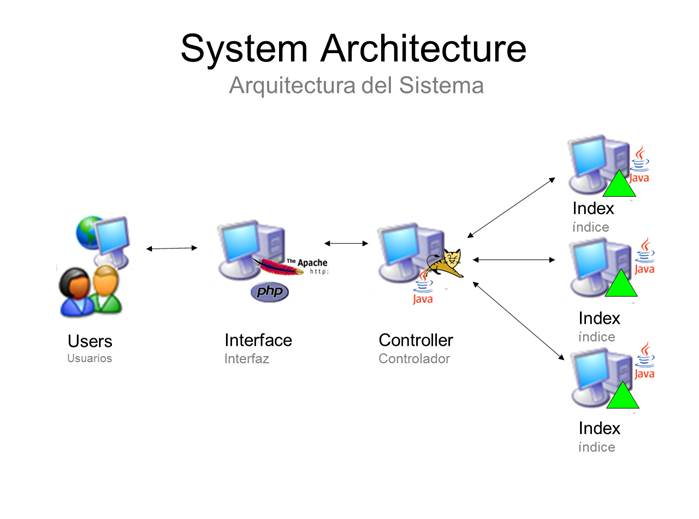
\includegraphics[scale=0.8]{img/ArquiteturaSistema.jpg}
\caption[Arquitetura do Sistema]{Arquitetura do Sistema}
\label{arquituraGeral}
\end{figure}



\subsection{Users}
...
\subsection{Interface}
...
\subsection{Controller}
...

\section{Considerações Finais}

\end{comment}

Na \autoref{sec:metodo} serão descrito os passos que serão realizados, os processos metodológicos adotados na pesquisa e como ocorrerá cada etapa do projeto. Já na \autoref{sec:estudo} serão abordados os elementos essenciais de um estudo de caso e a descrição de como será realizado o estudo de caso deste projeto de pesquisa. E, por fim, na \autoref{sec:classif} será realizado a classificação do projeto de pesquisa quanto aos gêneros identificados.

\section{Descrição do processo metodológico} \label{sec:metodo}

Nesta seção serão descritos os processos que serão realizados para se alcançar os objetivos geral e específicos estabelecidos. Na \autoref{fig:processo} serão ilustrados os passos básicos do processo feito para a aplicação deste projeto de pesquisa, contendo as fontes de dados, os passos e os resultado que serão gerados.

\subsection{Coleta de Dados}
Para este projeto de pesquisa, serão adotadas 4 fontes de dados. Esses dados coletados darão suporte para proposições que serão feitas para solucionar o problema. As quatro fontes de dados que serão usadas são: as respostas do Kahoot! de 2018.2, os resultados finais do processo de avaliação somativa de 2018.2, as respostas do Kahoot! de 2019.2 e os resultados parciais de 2019.2, as quatro na disciplina de Interface Humano-Computador.

\subsubsection{Respostas ao Kahoot!}
O Kahoot! é uma plataforma de GBL e foi descrita melhor na \autoref{sec:Kahoot!}. Na disciplina de Interface Humano-Computador (IHC), ela foi utilizada em 2018.2 e será utilizada em 2019.2 novamente. O Kahoot! tem um caráter fortemente formativo, sendo aplicado ao final de cada aula, com questões elaboradas pelo professor que abordem assuntos que foram ministrados na aula. 

As perguntas são de múltipla-escolha, tendo entre duas e cinco alternativas de respostas para o aluno. Neste projeto de pesquisa, serão usados os dados provenientes de respostas dadas pelos alunos aos questionários aplicados nas turmas de 2018.2 e 2019.2 da disciplina de Interface Humano-Computador da UFG, localizada em Jataí, sudoeste goiano. Na \autoref{fig:kahoot} é apresentado um \textit{Screenshot} de um exemplo de pergunta no Kahoot!

\subsubsection{Resultados parciais e finais da Avaliação Somativa}

O processo de Avaliação Somativa foi descrito na \autoref{sec:AvaSom}. O Kahoot! além de caráter formativo, ele também tem, ainda que pouco, caráter somativo. Além disso, serão utilizadas os resultados parciais e finais da disciplina de IHC para a analise dos resultados do projeto.

Da turma de 2018.2, serão usados os resultados finais da Avaliação Somativa, sendo que a disciplina já se encerrou, tendo apenas que coletar esses dados que estão armazenados. Já na turma de 2019.2, os resultados da Avaliação Somativa que serão usados são os parciais, consistindo de 2/3 da disciplina já realizada. O motivo desse ocorrido se dá em função do período que será necessário para obtenção e análise destes, visto que para se ter os resultados finais não haveria tempo hábil para realizar a análise completa destes, tendo assim uma perda. Acredita-se que, com esta porção de dados, será suficiente se ter resultados significativos e, assim, apresentar uma contribuição científica relevante.

\begin{figure}
    \centering
    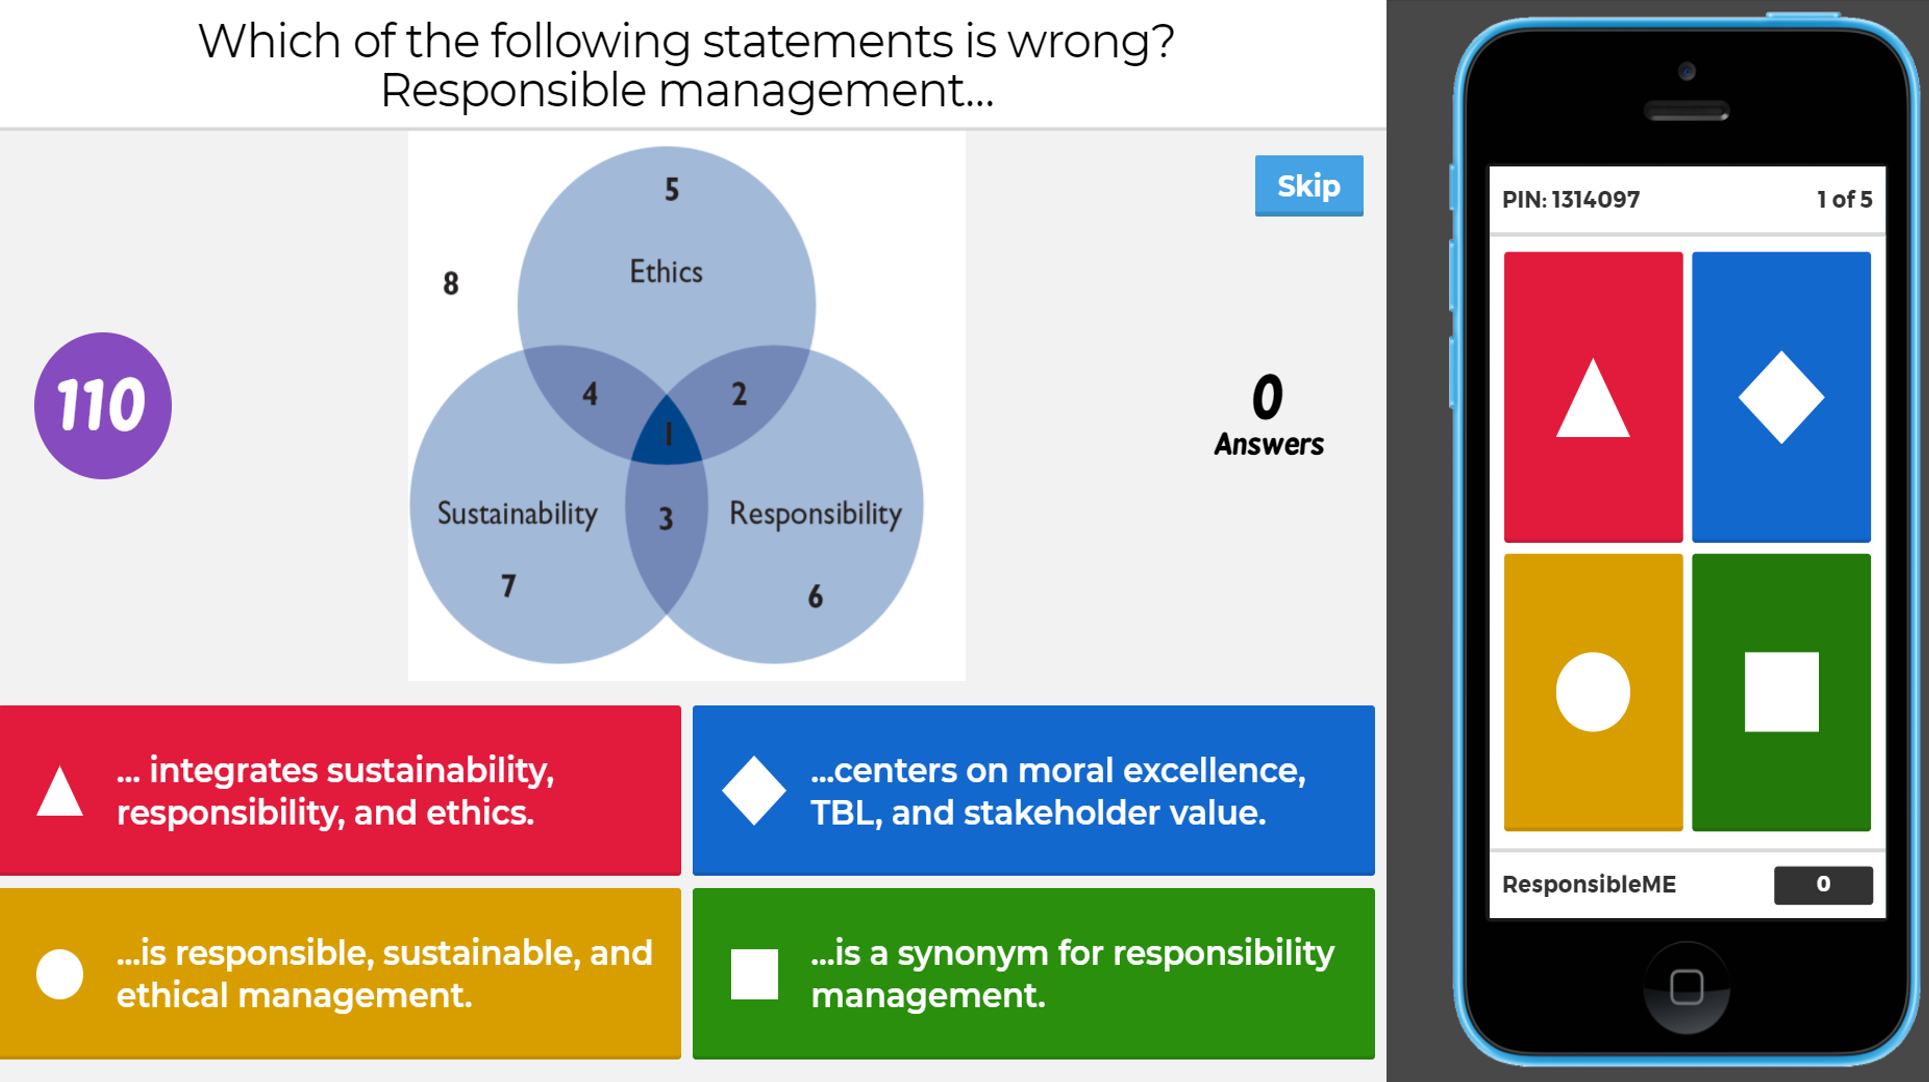
\includegraphics[width=0.7\textwidth]{modelo-monografia-rej-2018/img/KahootScreenshot.png}
    \caption{Exemplo de uma questão feita no Kahoot!}
    \label{fig:kahoot}
\end{figure}
 
\subsection{Projeto e Implementação da Rede Neural}

O projeto da Rede consiste em pegar um conjunto de dados de entrada, aplicar essa entrada em neurônios, onde esses reajustarão os pesos destas. A rede produz uma saída com a ``previsão'' da rede, aprovado ou reprovado --- sendo depois indicado o grau, provavelmente ou fortemente. O conjunto de entrada da Rede é composto por um vetor onde estarão as respostas dadas pelos alunos.

A Rede Neural Artificial será a técnica de aprendizagem de máquina usada por este projeto de pesquisa. A descrição desta foi feita na \autoref{sec:RNA}. Para isso, será projetada uma Rede Neural Artificial, adotando uma arquitetura de rede especifica.

A implementação da rede será feita na linguagem de programação \textit{Python}, que é uma linguagem interpretada, de \textit{script}, imperativa, orientada a objetos, funcional, de tipagem dinâmica e forte. Python é uma das opções mais comuns, quando se trata de Inteligência Artificial, talvez a que tenha mais biblioteca para Aprendizado de Máquina e Análise de Dados.

Uma destas bibliotecas é a TensorFlow, que é de código-aberto. É com ela que será criada e treinada a Rede Neural proposta por esta pesquisa. Essa biblioteca consiste em detectar e decifrar padrões e correlações, análogo à maneira com que o seres-humanos aprendem e raciocinam. 

{\color{red} [Por quê Python e TensorFlow?]}

\subsection{Treinamento da Rede Neural}

Como dito, o treinamento da Rede Neural será feito com a biblioteca TensorFlow na linguagem Python. Os dados usados para esse treinamento da rede serão os coletados das turmas de 2018.2 e 2019.2 de IHC. O projeto consiste em dividir as resposta pelo período em que elas foram aplicadas, sendo estes em 3 subdivisões.

A primeira rede será a rede com as entradas de dados dos primeiros 15 dias de aula, sendo estas entradas as respostas dadas nesse período às questões do Kahoot!, a segunda divisão será feita da mesma forma, porém as entradas serão as respostas dos primeiros 30 dias de aula. E, por fim, a última rede consistirá das respostas dadas nos primeiros 60 dias de aula.

Para melhor elucidação das arquiteturas, foram feitas 3 figuras para representar as redes que serão criadas, onde estão ilustradas como serão feitas as redes, e os conjuntos de entradas que serão adotadas. Na primeira rede (Ver \autoref{fig:rede01}), o conjunto de entrada será de 40 questões, sendo 10 por aula e 4 aulas no período de 15 dias. Na segunda rede (Ver \autoref{fig:rede02}), serão 30 dias e, consequentemente, o dobro de questões. E na terceira rede (Ver \autoref{fig:rede03}), o mesmo. Serão 160 questões em um período de 60 dias.

\begin{figure}
    \centering
    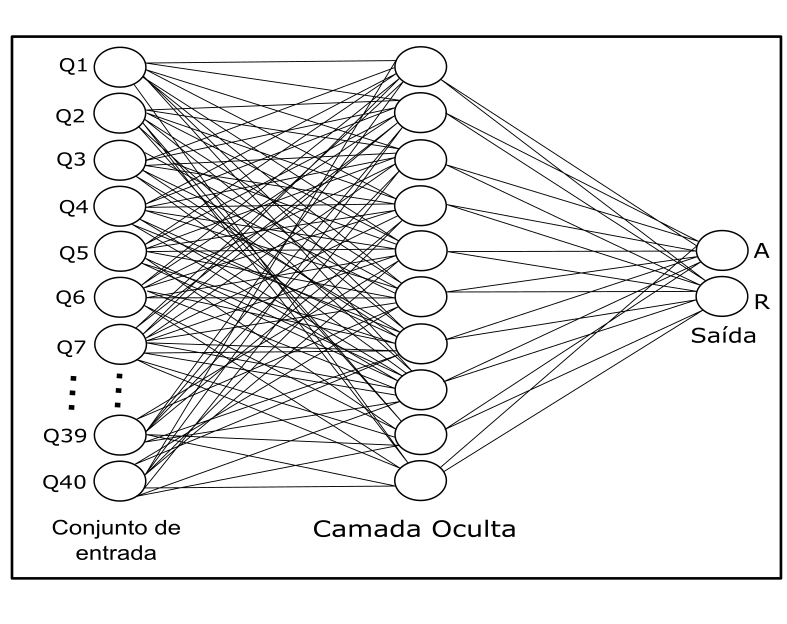
\includegraphics[width=0.9\textwidth]{modelo-monografia-rej-2018/img/rede01_15.png}
    \caption{Rede 01 - 15 dias de respostas}
    \label{fig:rede01}
\end{figure}

\begin{figure}
    \centering
    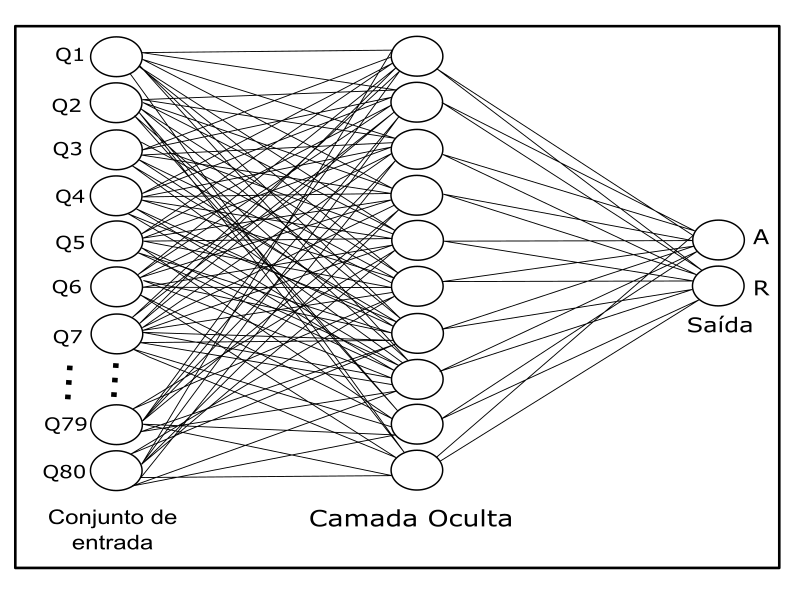
\includegraphics[width=0.9\textwidth]{modelo-monografia-rej-2018/img/rede02_30.png}
    \caption{Rede 02 - 30 dias de respostas}
    \label{fig:rede02}
\end{figure}

\begin{figure}
    \centering
    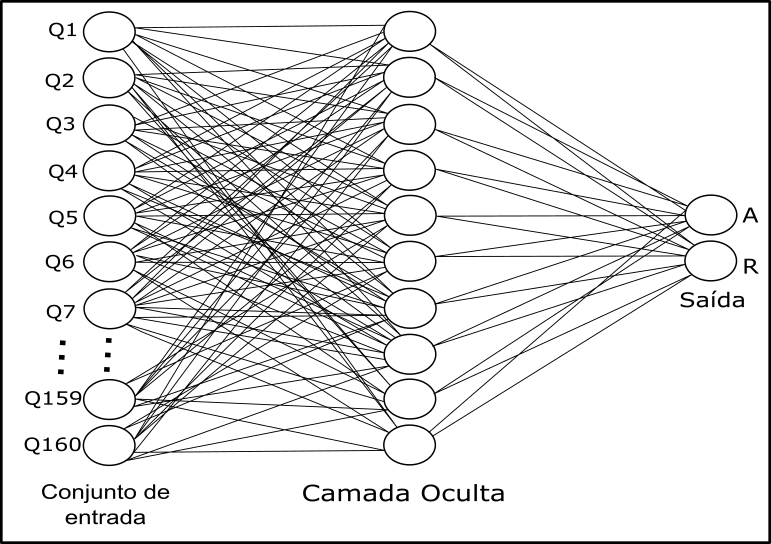
\includegraphics[width=0.9\textwidth]{modelo-monografia-rej-2018/img/rede03_60.png}
    \caption{Rede 03 - 60 dias de respostas}
    \label{fig:rede03}
\end{figure}

\subsection{Teste e Validação}

O teste e a validação serão feitos nas semanas subsequentes às estabelecidas para o treinamento, com as redes já com os ``neurônios'' com seu respectivo peso, feito através do processo de treino da rede. Ao fazer o teste e a validação, os alunos serão classificados em 4 grupos, que apresentarão o grau de risco e a situação dos alunos frente às previsões realizadas pela rede.

Serão usadas as respostas dos alunos ao Kahoot!. A rede fará a análise dos dados e verificará se há um padrão entre estes dados, se há uma correlação e, ao fazer as ligações ``sinápticas'' artificiais, como uma reprodução --- ou simulação --- do processo de raciocínio humano fará inferências quanto ao resultado acadêmico no processo de avaliação somativa, produzindo assim uma classificação deste aluno.

\subsection{Classificação dos alunos}
Após a análise ser feita pela Rede, o conjunto de saída apontará o aluno para que este integre um entre quatro grupos que serão estabelecidos. Os grupos seriam definidos como: Fortemente Reprovados (FR), Provavelmente Reprovados (PR), Provavelmente Aprovados (PA) e Fortemente Aprovados (FA). Esses níveis dizem respeito ao quão o aluno está propenso à reprovar. Pensando em um plano cartesiano, seria como se no eixo das abcissas fosse posto esses níveis classificatórios. Nessa analogia, quanto mais à esquerda o aluno fosse classificado, maior seria a chance do aluno ser reprovado na disciplina, quanto mais à direita o aluno fosse classificado, maior seria a chance desse aluno ser aprovado.

A questão que aparece ao se fazer essa classificação é a seguinte: ``Um aluno não pode ser classificado de forma errada?''. Sim, ele pode, e isso é descrito por quatro conceitos (ver \autoref{fig:Venn}) importantes de serem definidos neste projeto de pesquisa, que são:

\begin{itemize}
    \item \textbf{Falsos-negativos (FN)}: Com os resultados alcançados pela rede, alunos podem ser classificados como se não estivessem no grupo de risco de reprovação, mas acabam reprovando. São os chamados falsos-negativos.
    \item \textbf{Falsos-positivos (FP)}: Os alunos podem ainda ser classificados como alunos em situação de risco de reprovação, mas ao final da disciplina alguns desses alunos serem aprovados, constatando assim os chamados Falsos-positivos.
    \item \textbf{Verdadeiros-negativos (VN)}: Os alunos classificados como não pertencentes ao grupo de risco de reprovação e que acabam aprovados, sendo assim corretamente classificados previamente, são denominados Verdadeiros-negativos.
    \item \textbf{Verdadeiros-positivos (VP)}: Já os alunos que são classificados como alunos em situação de risco de reprovação e, ao final da disciplina, acabam realmente reprovando, são chamados de Verdadeiros-positivos.
\end{itemize}

\begin{figure}
    \centering
    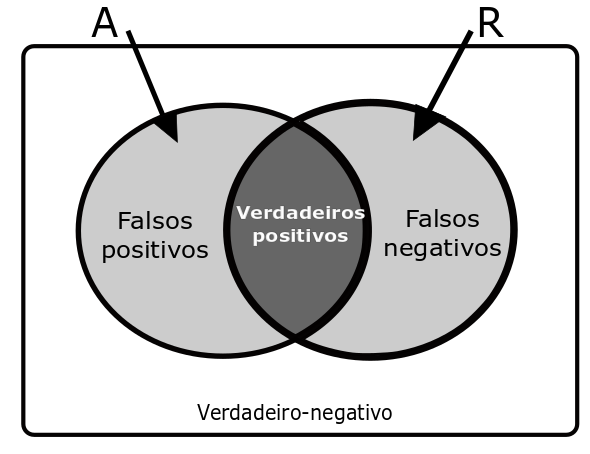
\includegraphics[width=0.9\textwidth]{modelo-monografia-rej-2018/img/DiagramaVenn.png}
    \caption{Diagrama de Venn para Falsos/verdadeiros negativos e positivos}
    \label{fig:Venn}
\end{figure}

\subsection{Análise dos Resultados}
\label{ss:analise}
Após a produção dos resultados e e classificação da situação dos alunos, o passo seguinte do projeto de pesquisa é analisar os resultados para saber se estes foram satisfatório e estão de acordo com o esperado. Para isso serão usados como métrica os índices de Precisão, Acurácia e Cobertura (\textit{Recall}). As formalizações propostas em outras literaturas para essas três métricas são as seguintes:


$Acurácia = \frac{VP+VN}{VP+VN+FP+FN}*100$

$Precisão = \frac{VP}{VP+FP}*100$

$\textit{Recall} = \frac{VP}{VP+FN}*100$

\begin{figure}
    \centering
    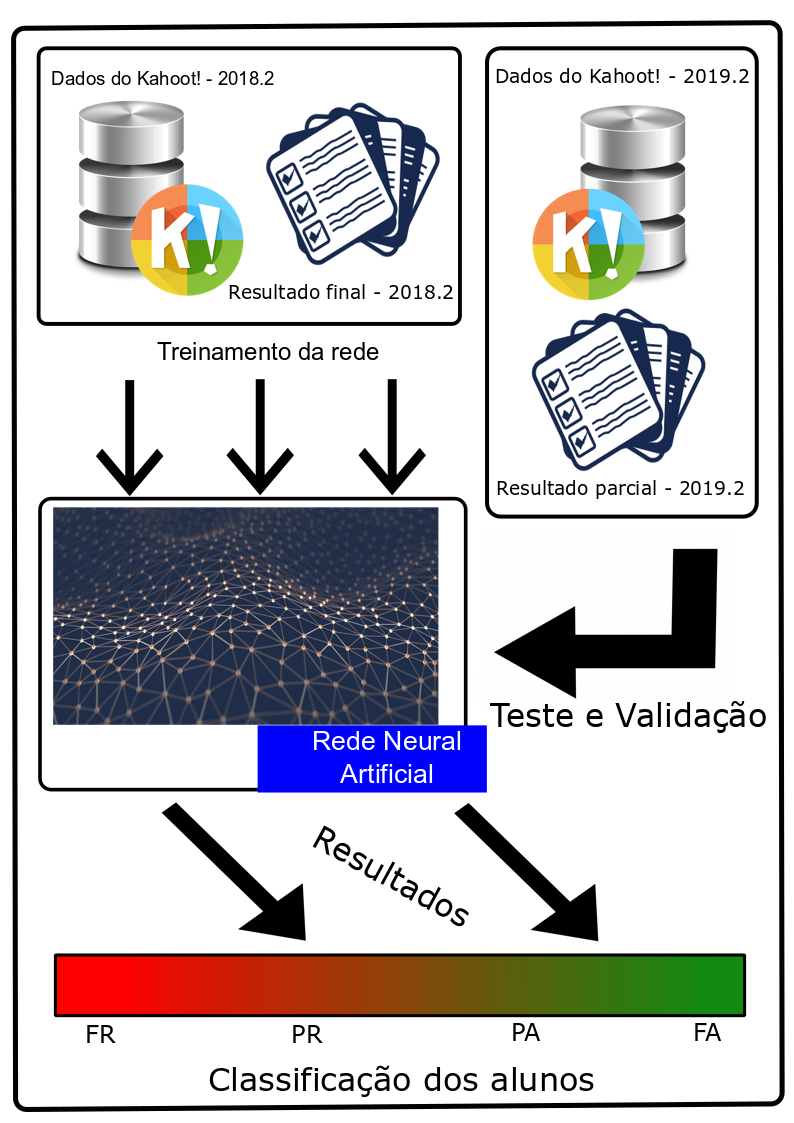
\includegraphics[width=0.5\textwidth]{modelo-monografia-rej-2018/img/ProcessoMetodologico.png}
    \caption{Diagrama esquemático dos processos do projeto de pesquisa}
    \label{fig:processo}
\end{figure}


\section{Estudo de caso}
\label{sec:estudo}
Um estudo de caso é uma investigação empírica que investiga um fenômeno contemporâneo dentro de seu contexto da vida real, especialmente quando os limites entre o fenômeno e o contexto não estão claramente definidos \cite{yin2001planejamento}. Esta investigação enfrenta uma situação tecnicamente única em que haverá muito mais variáveis de interesse do que fonte de dados, e, como resultado, (1) baseia-se em fontes de evidências, com os dados precisando assimilar-se a trabalhos correlatos, e, como outro resultado, (2)beneficia-se do desenvolvimento prévio de proposições teóricas para conduzir a coleta e análise de dados.

\subsection{Descrição do estudo de caso}
Este é um estudo de caso único holístico, utilizando uma estratégia exploratória. A justificativa deste estudo reside no caso revelador que é o uso de RNA na predição de desempenho acadêmico dos alunos em Educação de Computação no Brasil. Os estudos do levantamento bibliográfico concentram-se principalmente em países da América do Norte, Europa e Oceania, como descrito no \autoref{sec:TR}.
Segundo \citeonline{yin2001planejamento}, um estudo de caso contém, em especial, cinco componentes importantes de um projeto de pesquisa que serão descritos a seguir.

%\subsection{Questões do estudo}
Para nortear este estudo de caso, a questão principal levantada foi \textbf{Q1: ``Quais são os resultados ao se utilizar a RNA na previsão de alunos em situação de risco de reprovação em Educação de Computação no contexto Brasileiro?''}

%\subsection{Proposições} \label{sec:HS}
As seguintes proposições foram estabelecidas a fim de serem investigadas. A Proposição 1 \textbf{(P1): ``A precisão da RNA alcançou um nível satisfatório.''}, Proposição 2 \textbf{(P2): ``A acurácia da RNA teve um desempenho satisfatório''} e Proposição 3 \textbf{(P3): ``A cobertura (\textit{Recall}) atingiu um nível satisfatório''}.

\subsection{Unidade de análise e Coleta de Dados}
A unidade de análise do estudo é a turma de 2019.2 da disciplina de Interface Humano-Computador do Bacharelado em Ciência da Computação da Universidade Federal de Jataí, localizada no sudoeste goiano.

A coleta dos dados terá quatro fontes: as respostas dos alunos no Kahoot! de 2018.2 (F1), o resultado final do processo de avaliação somativa dos alunos da turma de 2018.2 (F2), as respostas ao Kahoot! de 2019.2 (F3) e o resultado parcial da avaliação formativa dos alunos da turma de 2019.2 (F4). As duas turmas são da disciplina de Interface Humano-Computador. 

As respostas são dadas pelos alunos, no final de cada aula, às perguntas elaboradas pelo professor que ministra a disciplina, através da ferramenta de tecnologia educacional, ``Kahoot!'', que foi descrita na seção \ref{sec:Kahoot!} e os resultados parciais e finais no processo de avaliação somativa - aprovado ou reprovado - obtidos por esses alunos.

Ao final da disciplina e do processo de avaliação somativa, os alunos alcançam certo resultado - aprovado ou reprovado - que será um dos dados que formará o conjunto que será analisado.

\subsection{Análise dos Dados}
Para demonstrar a ligação entre os dados coletados e as proposições estabelecidas, serão adotadas três métricas, os resultados de \textbf{precisão}, \textbf{Acurácia} e Cobertura (\textit{Recall} obtidos por trabalhos correlatos. Os dados coletados servirão como suporte para a proposição através da métrica adotada. Se os resultados alcançados forem próximos às métricas, podemos dizer que a previsão feita pela RNA atingiu um nível satisfatório. Mais detalhes serão descritos a seguir. Para melhor compreensão, os conceitos de Acurácia e Precisão são importantes de serem explicados e diferenciados e serão na \autoref{dif}. As fórmulas que os descrevem já foram explicitadas na \autoref{ss:analise}.

As métricas usadas serão usadas como suporte para dizer se os resultados alcançados neste projeto satisfizeram as proposições estabelecidas, ou seja, os níveis alcançados foram satisfatórios. Para definir os valores estabelecidos, tomaremos como base os valores obtidos para os atributos de métrica descritos, evidenciando resultados concretos já alcançados. Os trabalhos em questão serão os Trabalhos Relacionados da \autoref{sec:TR}, onde se alcançaram níveis próximos ao que será estabelecido para este, que terá uma margem de consideração. Formalmente, podemos dizer que as métricas que servirão de base, serão:

$Acurácia = \left \{ x | x >= 70\% \right \}$

$Precisão = \left \{ y | y >= 75\% \right \}$

;$Recall = \left \{ z | z >= 70\% \right \}$
\subsubsection{Diferença entre Precisão e Acurácia} \label{dif}

\textbf{Precisão} se define como a proximidade entre os valores obtidos pela repetição do processo de mensuração. Quanto menor é a diferença destes valores, melhor é a precisão. \textbf{Acurácia} se define como a proximidade da medida em relação ao verdadeiro valor, um valor definido, que se deseja obter. Quanto mais próximo do valor real, melhor é a acurácia. A \autoref{fig:PrecAcur} esclarece isso de maneira bem didática.

\begin{figure}
    \centering
    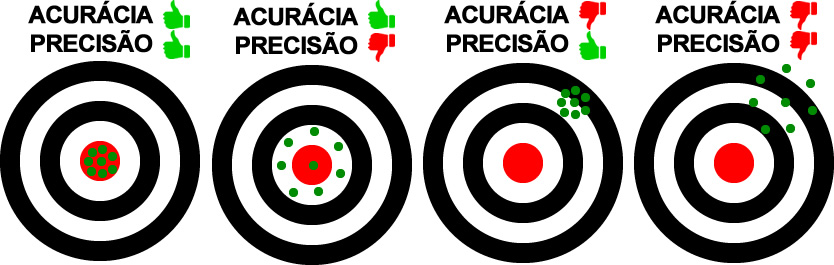
\includegraphics[width=0.9\textwidth]{modelo-monografia-rej-2018/img/PrecisaoAcuracia.jpg}
    \caption{Diferença entre Acurácia e Precisão}
    \label{fig:PrecAcur}
\end{figure}

\section{Classificação da pesquisa}
\label{sec:classif}
A classificação desse projeto de pesquisa pode ser feito em termos de gêneros da mesma. Estes gêneros dizem respeito à natureza, os objetivos, os procedimentos, o objeto e à forma de abordagem desta.

\subsection{Gêneros de Pesquisa}

{\color{red} COLOCAR FRASE}

\subsubsection{Quanto à natureza}
Empírica, pois a pesquisa dedica-se recolher dados diretamente da realidade do objeto de estudo, mensurar a realidade, formular observações e propor transformações do mesmo enquanto objeto de investigação, mas não intervem de forma concreta no ambiente durante o trajeto da pesquisa.

\subsubsection{Quanto aos objetivos}
Pesquisa exploratória: Apesar de haverem pesquisas em relação à métodos para a predição dos resultados do processo de avaliação somativa --- aprovado ou reprovado ---, há a necessidade de se relatar casos no Brasil, que ocorram experimentos da aplicação desses métodos no processo de avaliação de aprendizagem, identificando alunos em situação de risco.

\subsubsection{Quanto aos procedimentos}
Pesquisa de Campo: Todos os procedimentos que serão usados nesta pesquisa serão derivados de coletas de dados realizadas em fontes diretas. Desta forma, esta pesquisa quantos aos procedimentos é de campo, pois baseia-se em dados coletados no local da ocorrência dos fatos.

\subsubsection{Quanto ao objeto}
Pesquisa de campo: O principal objeto desta pesquisa é justamente a identificação prévia de alunos em risco de reprovação e o uso de Redes Neurais Artificiais como método preditivo. O conceito sobre o objeto, o problema relacionado ao mesmo, assim como a justificativa, são oriundos de uma coleta de dados realizada em local, tornando esta pesquisa de campo quanto aos objetos.

\subsubsection{Quanto à forma de abordagem}
Pesquisa quantitativa: Serão coletadas as respostas dadas pelos alunos, analisando os dados gerados, com o modelo de Rede Neural criado, e produzindo, assim, uma saída classificada.

\chapter{Implementação ou Construção}\label{cap:implementacao}
\section{Introdução}
Este capítulo apresenta a criação e desenvolvimento da contribuição ao método, baseados na metodologia apresentada nos capítulos anteriores. Se for desenvolvimento de software, os pseudocódigos e/ou algoritmos devem ser detalhados. Em alguns casos o mais correto é apresentar um formalismo matemático do que foi elaborado, permitindo aos avaliadores maior possibilidade da verificação da contribuição.

\section{Metodologia de Desenvolvimento}
\section{Pseudocódigos}
\section{Algoritmos}

\section{Considerações Finais}





\chapter{Funcionamento ou Demonstração}\label{cap:funcionamento}
\section{Introdução}
Nesta seção é apresentado o funcionamento daquilo que foi planejado no capítulo 4 (metodologia), construído no capítulo 5 (construção). Em muitos casos é necessário usar um estudo de caso para apresentar a contribuição (neste modelo de pesquisa o estudo de caso não é tão importante e sim a contribuição). Outros casos, quando existe uma preocupação com o estudo de caso, ligados diretamente ao objeto de estudo que deu origem ao problema, o mesmo (estudo de caso) pode ser apresentado no capítulo 4 (descrição necessária para definição da solução) e novamente nesta seção (aplicação da solução). 


\section{Exemplo de Aplicação}

\section{Considerações Finais}




\chapter{Avaliação e Testes}\label{cap:analise}
\section{Introdução}
Neste capítulo é apresentada uma análise da aplicação ou uso do que foi construído e demonstrado no capítulo anterior. Esta análise pode ser realizada usando normas (ISO/EIC) já estabelecidas. Pode ser por meio de testes de laboratório, pode ser simulada, pode ser aplicada em um contexto (universo/população/amostragem) real. E, também pode ser por meio da criação de uma metodologia própria para a análise.

\section{Ambiente Experimental}

\section{Análise dos Resultados Obtidos}

\section{Métricas}

\section{Considerações Finais}





\chapter{Conclusões e Trabalhos Futuros}\label{cap:conclusao}
\section{Introdução}
Este capítulo tem como objetivo apresentar os principais pontos discutidos no trabalho, relacionar os possíveis trabalhos futuros advindos desta pesquisa e avaliar a principal contribuição deste trabalho para a área científica.





\section{Conclusões}

As conclusões devem estabelecer uma descrição sucinta e sintética daquilo que o autor concluiu ao desenvolver sua pesquisa. Deve haver um cuidado para que a mesma não seja óbvia e também que não seja impossível de identificar no texto. Conclusões sobre um ou outro tipo de tecnologia usada, conclusões sobre caminhos que foram tomados na condução da pesquisa são importantes. E, cabe ressaltar que este texto é do autor, portanto não cabe nesta seção a inserção de referências bibliográficas.

\subsection{Quanto à área aplicada}




\subsection{Quanto à área específica}



\section{Trabalhos futuros}


Em todo trabalho científico, vários caminhos podem ser estabelecidos. Porém cabe geralmente ao autor definir um único para viabilizar a produção e divulgação da sua pesquisa. Estes outros caminhos podem ser apresentados nesta seção, detalhando claramente os motivos da não escolha pelos mesmos. 
Também muito importante nesta seção, é vislumbrar o que ainda pode ser realizado na sequência do próprio trabalho. Toda pesquisa é provavelmente infinita, o que a classifica como concluída, é apenas um ponto de parada para sua divulgação. Portanto, outras contribuições são e serão sempre passíveis. É exatamente isso que cria a evolução, o desenvolvimento e gera inovação. Na área da Ciências Exatas, o termo “Estado da Arte” dá a exatidão desta sequencia. 


\section{Considerações finais}




% ----------------------------------------------------------
% ELEMENTOS PÓS-TEXTUAIS
% ----------------------------------------------------------
\postextual
% ----------------------------------------------------------

% ----------------------------------------------------------
% Referências bibliográficas
% ----------------------------------------------------------
\bibliography{bib}

% ----------------------------------------------------------
% Glossário
% ----------------------------------------------------------
%
% Consulte o manual da classe abntex2 para orientações sobre o glossário.
%
%\glossary

% ----------------------------------------------------------
% Apêndices
% ----------------------------------------------------------




% ----------------------------------------------------------
% Anexos
% ----------------------------------------------------------

% ---
% Inicia os anexos
% ---
% ---
% Inicia os anexos
% ---
\begin{anexosenv}

% Imprime uma página indicando o início dos anexos
\partanexos

\chapter{Exemplo de Formulário}\label{anexo:formAluno}

Este formulário tem como objetivo ...:

1.	Quanto ...?\\


2.	Qual o nível...?\\
Ruim 0 (   )      1 (   )     2 (   )      3 (    )     4 (   )	Ótimo\\


3.	Qual o nível de ...?\\
Ruim 0 (   )      1 (   )     2 (   )      3 (    )     4 (   )	Ótimo\\	



\end{anexosenv}

%---------------------------------------------------------------------
% INDICE REMISSIVO
%---------------------------------------------------------------------
%\phantompart
\printindex
%---------------------------------------------------------------------

\end{document}
